
\section{Experiments}~
In the following, we compare Python implementations of our algorithms,
the \naive\ MH algorithm (algorithm~\ref{alg:MH_naive}) and its symmetrized
improvement (algorithm~\ref{alg:MH_improved}), against 
baselines like Gibbs sampling (algorithm~\ref{alg:MJP_gibbs}),
and particle MCMC~\cite{Andrieu10}. We look at different variants
of these algorithms, corresponding to different uniformizing Poisson 
rates, and different number of particles.
For schemes involving simple uniformization in the manner of~\cite{RaoTeh13}, we 
set $\Omega(\theta) = \kappa \max_s A_s(\theta) $ with $\kappa$  equal to 
$1.5, 2$ and $3$. When the uniformizing rate depends on both the current and 
proposed parameter, we consider two settings
 $\Omega(\theta, \theta^*) = \kappa (\max A(\theta) + \max A(\theta^*))$ 
 ($\kappa = 1$ and $2$), and 
$\Omega(\theta, \theta^*) = \kappa \max(\max A(\theta), \max A(\theta^*))$
($\kappa=1.5$). 
Unless specified, our results were
obtained from $100$ independent MCMC runs, each consisting of $10000$ iterations.
We found particle MCMC to be more computationally intensive, and limited each 
run to $3000$ iterations, the number of particles being $5, 10$ and $20$. 

% We also considered exploiting gradient information of the target distribution to 
% apply Hamiltonian Monte Carlo (HMC)~\cite{Neal2010}. In particular, the forward 
% pass of FFBS allows us to also calculate the gradient of the log-probability with
% respect to the MJP parameters. We can exploit this information for more directed
% explorations of parameter space than a random-walk algorithm. Of course, this 
% comes at a higher computational cost. We evaluate HMC with the number of leapfrog
% steps taking values in $1, 3, 5$ or $10$, and the leapfrog stepsize taking values 
% in $0.02, 0.05$ and $0.1$. 

For each run of each MCMC algorithm, we calculated the effective sample size 
(ESS) of the posterior samples of the MJP parameters using the R package 
\texttt{rcoda}~\cite{Rcoda2006}. This estimates the number of independent 
samples returned by the MCMC algorithm, and dividing this by the runtime of a 
simulation gives the ESS per unit time. We used this measure to compare 
different MCMC samplers/different parameter settings of each sampler.

% \begin{algorithm}[!ht]
%    \caption{Generic Gibbs sampling for MJPs for Gamma priors}
%    \label{alg:Generic Gibbs}
% \begin{algorithmic}
%    \State {\bfseries Input:} observations $y_{[t_0, t_{k+1})}$
%    \State Initialize, $i = 0$
%    \\ (a) Set $\alpha(0), \beta(0)$ arbitrarily and set current trajectory $[S,T](0)$ arbitrarily.\\
%     (b) Uniformize $[S,T](0)$, to get virtual jumps $U$.
%    \Repeat
%    \For{$i=1$ {\bfseries to} $N$}
%     \State (a) Sample $U(i) \sim P( U | \beta(i - 1), \alpha(i - 1), S(i - 1), T(i - 1), y)$.\\	
%     \State (b) Use FFBS algorithm to  sample states given all the jump times(both true jumps and virtual jumps).
% (i.e. $V(i) \sim P(V |  \beta(i - 1), \alpha(i - 1), W(i ), y).$) Then delete all the virtual jumps to get $S(i), T(i) .$\\
%     \State (c) Propose $\beta^* \sim q(.| \beta(i -1))$.\\
%       Set $\beta(i) = \beta^*$, with probability $P_{acc} = 1 \wedge \frac{P(\beta^* |S(i), T(i))}{P(\beta(i - 1) |S(i), T(i))} \frac{q(\beta(i - 1)|\beta^*)}{q(\beta^*|\beta(i - 1))}$;\\Otherwise set $\beta(i) = \beta(i-1)$.\\	  
%     \State (d) Sample $\alpha(i) \sim P(. | \beta(i), S(i), T(i), y)$.\\ It is a $Gamma(\mu + N, \lambda + \sum_{0}^NF_{S_i}(\beta)(t_{i + 1} - t_i))$ distribution actually.\\
%     \EndFor
%     \Until{$ i = N$ }
%  \end{algorithmic}
%  \end{algorithm}

\subsection{A simple synthetic MJP}
  \begin{figure}[H]
  \centering
  \begin{minipage}[!hp]{0.45\linewidth}
  \centering
    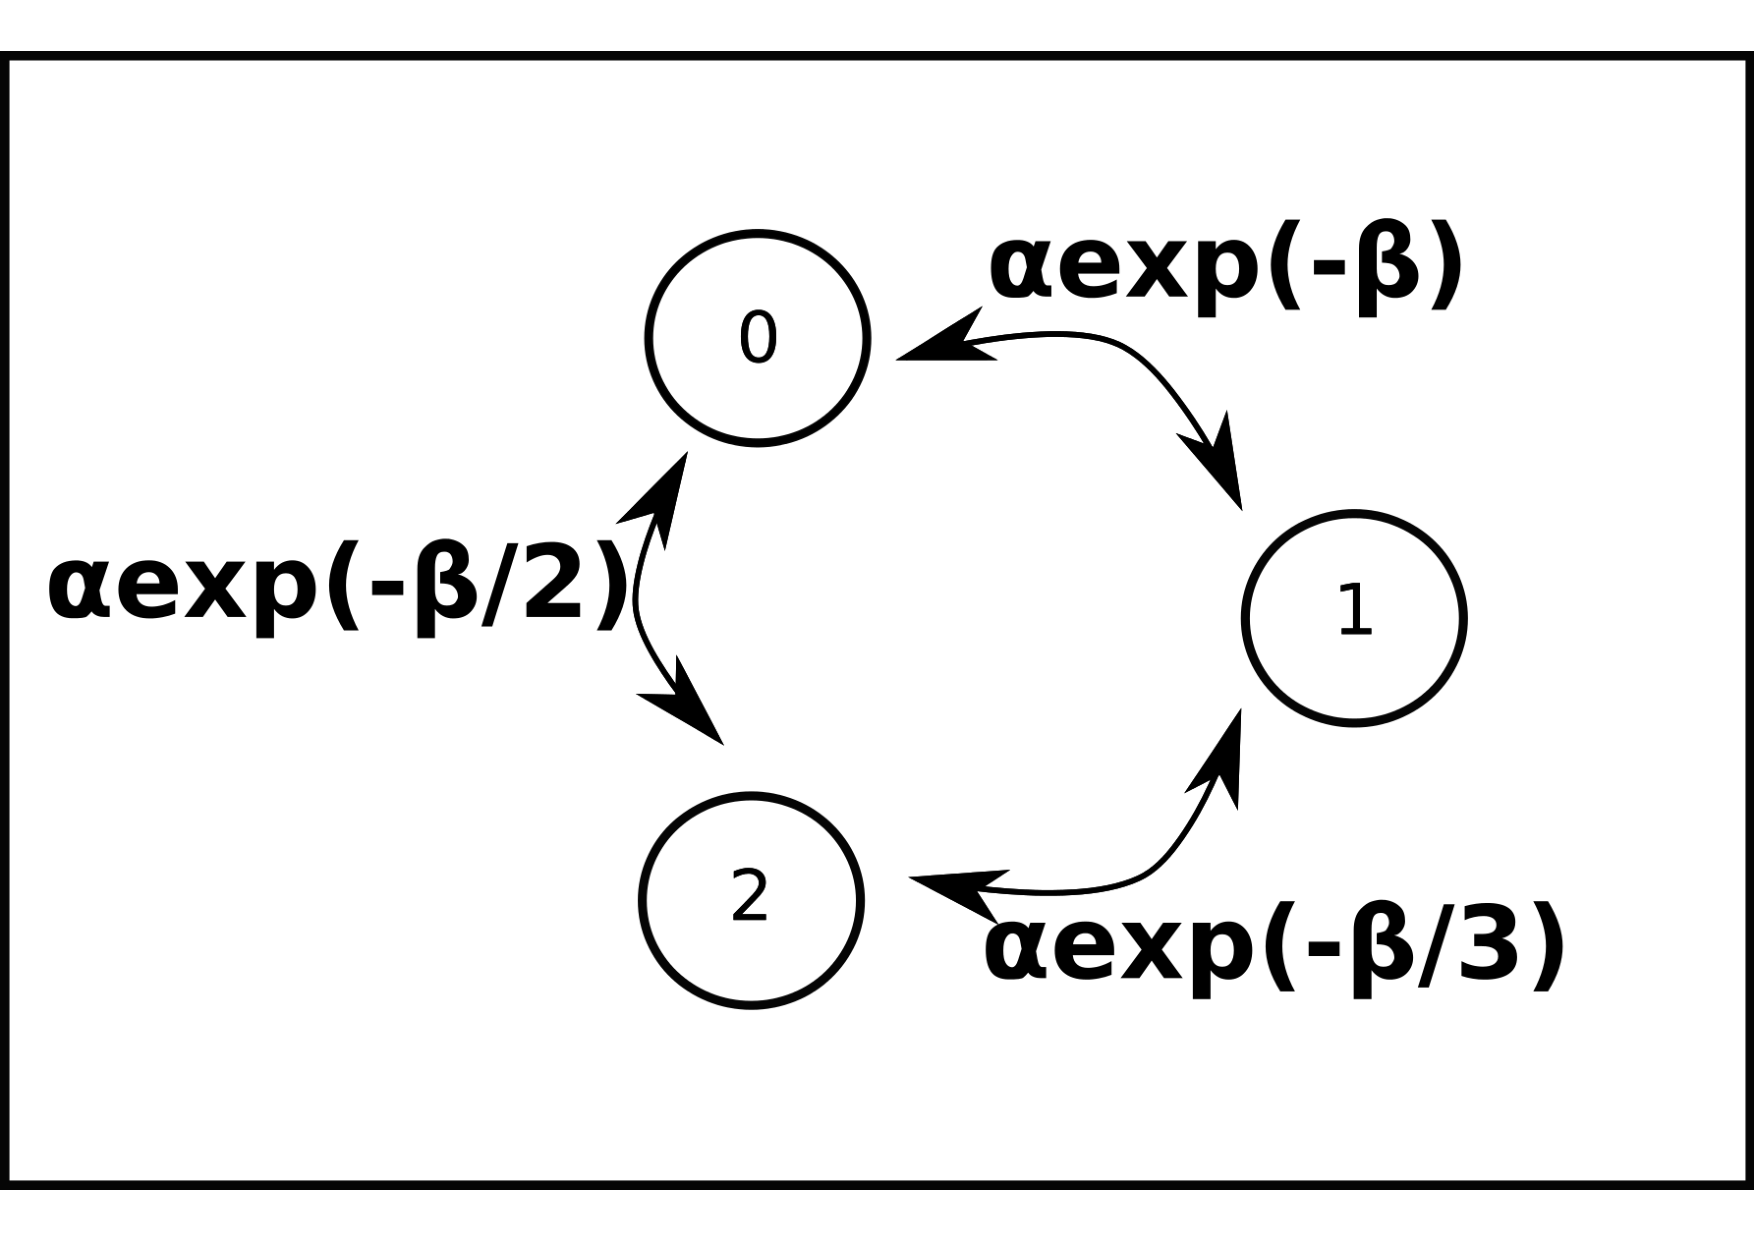
\includegraphics [width=0.70\textwidth, angle=0]{figs/exp_model.pdf}
      \end{minipage}
    \caption{A 3-state MJP with exponentially decaying rates}
    \label{fig:exp_model}
  \end{figure}

% \noindent Assume: $S = [S_0,S_1, ...,S_N] \;, T = [t_0(t_{start}), t_1,...,t_N, t_{N+1}(t_{end})]$, and y as observations.\\
% We consider a specific structure of rate matrix $A$. $A_{ij} = \alpha f_{ij}(\beta), \; i \neq j$. $A_{ii} = -\sum_{j \neq i} A_{ij}$. $0 \leq f_{ij} \leq 1$. Denote $F_i(\beta) = \sum_{j \neq i} f_{ij}(\beta)$.\\
% \begin{align*}
% P(s_0, S, T | \alpha, \beta) &= \pi_0(s_0)\prod_{i = 1}^N A_{S_{i - 1}S_i} \exp(- \int_{t_{start}}^{t_{end}} |A_{S(t)}| dt)\\
% &= \pi_0(s_0) \alpha^N \prod_{i = 1}^N f_{S_{i - 1}S_i} \exp(-\alpha  \sum_{i = 0}^{N} F_{S_i}(\beta)(t_{i + 1} - t_i))\\
% \end{align*} 
\noindent Consider an MJP with two parameters $\alpha$ and $\beta$, 
transitions between states $i$ and $j$ having rate $\alpha \exp(-\beta/(i+j))$.
We consider three settings: $3$ states (figure~\ref{fig:exp_model}),
$5$ states, and $10$ states.
We place Gamma$(\alpha_0,\alpha_1)$, and Gamma$(\beta_0, \beta_1)$ priors on 
the parameters $\alpha$ and $\beta$, with $(\alpha_0,\alpha_1,\beta_0,\beta_1)$ 
having values $(3,2,5,2)$ respectively. For each run, we draw random parameters 
from the prior to construct a transition matrix $A$, and placing a uniform 
distribution over states at time $0$, simulate an MJP trajectory.
We simulate observations uniformly at integer values on the time interval 
$[0, 20]$. Each observation is Gaussian distributed with mean equal to the state
at that time, and variance equal to $1$.  For the Metropolis-Hastings proposal, 
we used a lognormal distribution centered at the current parameter value, with 
a user-specified variance.
%\vinayak{We studied our MH sampler, for three setting of $k$}.  
% %\begin{align*}
% %P(\alpha, \beta | s_0, S, T ) \propto \alpha^N \prod_{i = 1}^N f_{S_{i - 1}S_i} \exp(-\alpha  \sum_{i = 0}^{N} F_{S_i}(\beta)(t_{i + 1} - t_i)) p_1(\alpha)p_2(\beta)\\
% %\end{align*}
% %If we assume the priors of $\alpha$, $\beta$ are $Gamma(\mu, \lambda)$, $Gamma(\omega, \theta)$, then the posterior will have a simper form as follows. 
% \begin{align*}
% P(\alpha, \beta | s_0, S, T ) = C \alpha^{\mu + N - 1}\exp(-\alpha (\lambda + \sum_{i = 0}^{N} F_{S_i}(\beta)(t_{i + 1} - t_i))) \prod_{i = 1}^N f_{S_{i - 1}S_i}  \beta ^{\omega - 1} \exp(-\theta \beta)\\
% \end{align*}
% We notice that given $\beta,\; S,\; T$, $\alpha$ is distributed as a $Gamma$ distribution.\\
% $\alpha | \beta, S, T, y  = \alpha | \beta, S, T \sim Gamma(\mu + N, \lambda + \sum_{0}^NF_{S_i}(\beta)(t_{i + 1} - t_i))$.\\
% There is no conjugate distribution to sample $\beta \sim P(\beta| s_0, S, T)$. We will have to use Metropolis Hasting within Gibbs to sample $\beta$. The target distribution is the following one.
% $$ P(\beta | S, T) = C \frac{\prod_{i = 1}^N f_{S_{i -1}S_i}(\beta)\beta^{\omega - 1} \exp(-\theta \beta)}{(\lambda + \sum_{i = 0}^{N} F_{S_i}(\beta)(t_{i + 1} - t_i))^{\mu + N}}.$$
% Such doubling might slow the mixing of the Markov chain. We can apply our Metropolis Hasting algorithm on this model.

\noindent \textbf{Results:}
  \begin{figure}%[b]
  \centering
  \begin{minipage}[!hp]{0.45\linewidth}
  \centering
    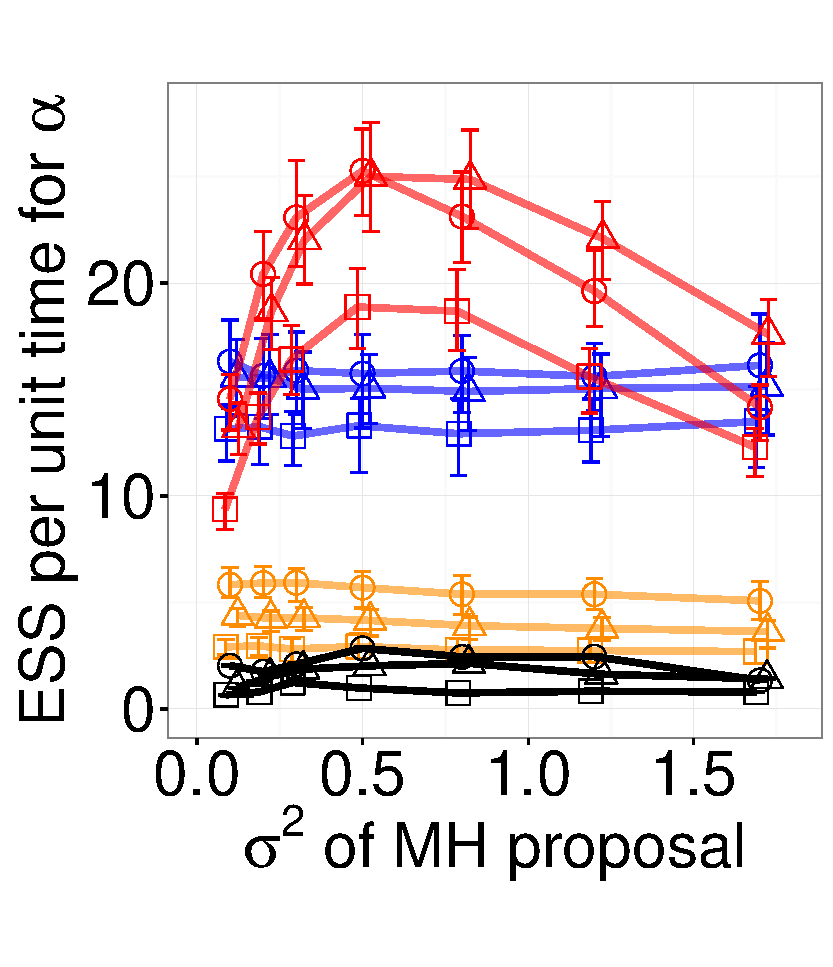
\includegraphics [width=0.90\textwidth, angle=0]{figs/exp_3_alpha.pdf}
      \end{minipage}
  \begin{minipage}[hp]{0.45\linewidth}
  \centering
    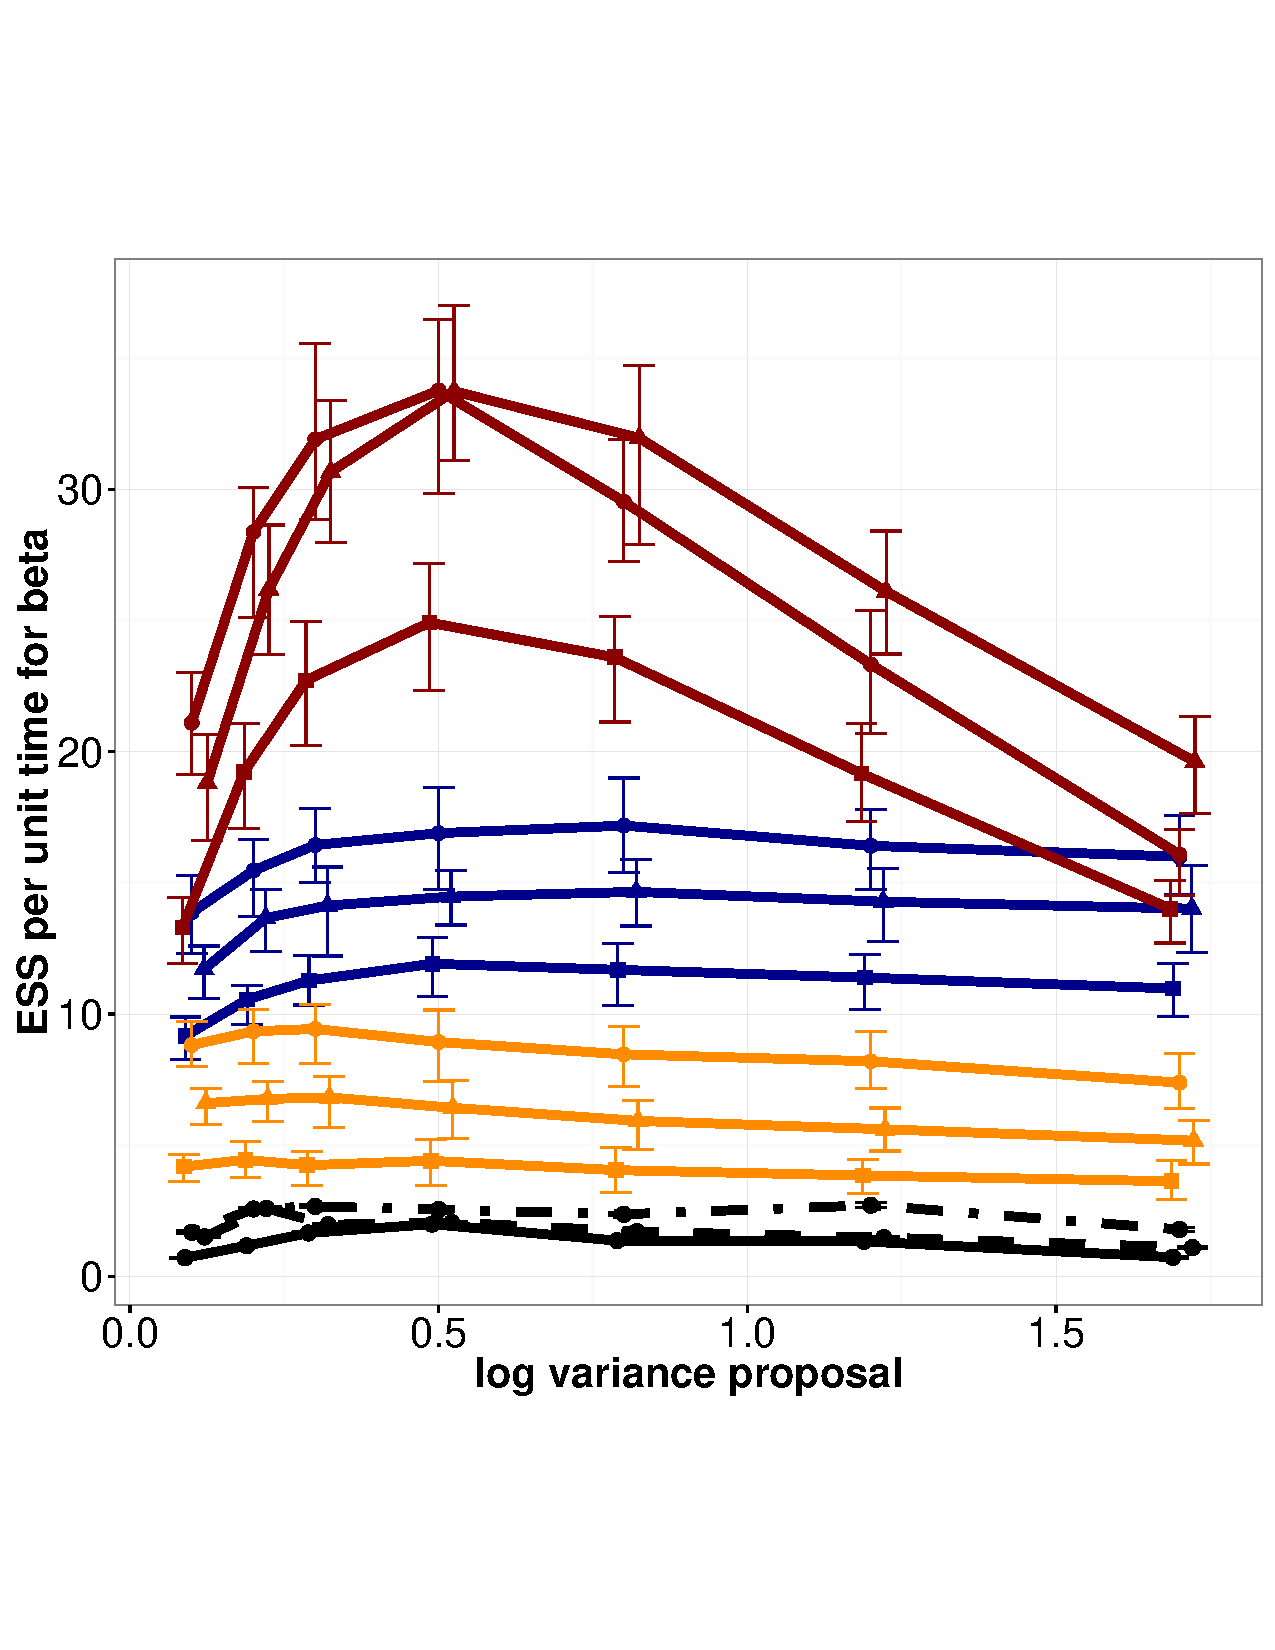
\includegraphics [width=0.90\textwidth, angle=0]{figs/exp_3_beta.pdf}
    \vspace{-0 in}
  \end{minipage}
    \caption{ESS/sec for exp model (dim 3). The left is for $\alpha$, and the right is for $\beta$.}
     \label{fig:ESS_EXP_D3}
  \end{figure}
  \begin{figure}%[b]
  \centering
  \begin{minipage}[!hp]{0.45\linewidth}
  \centering
    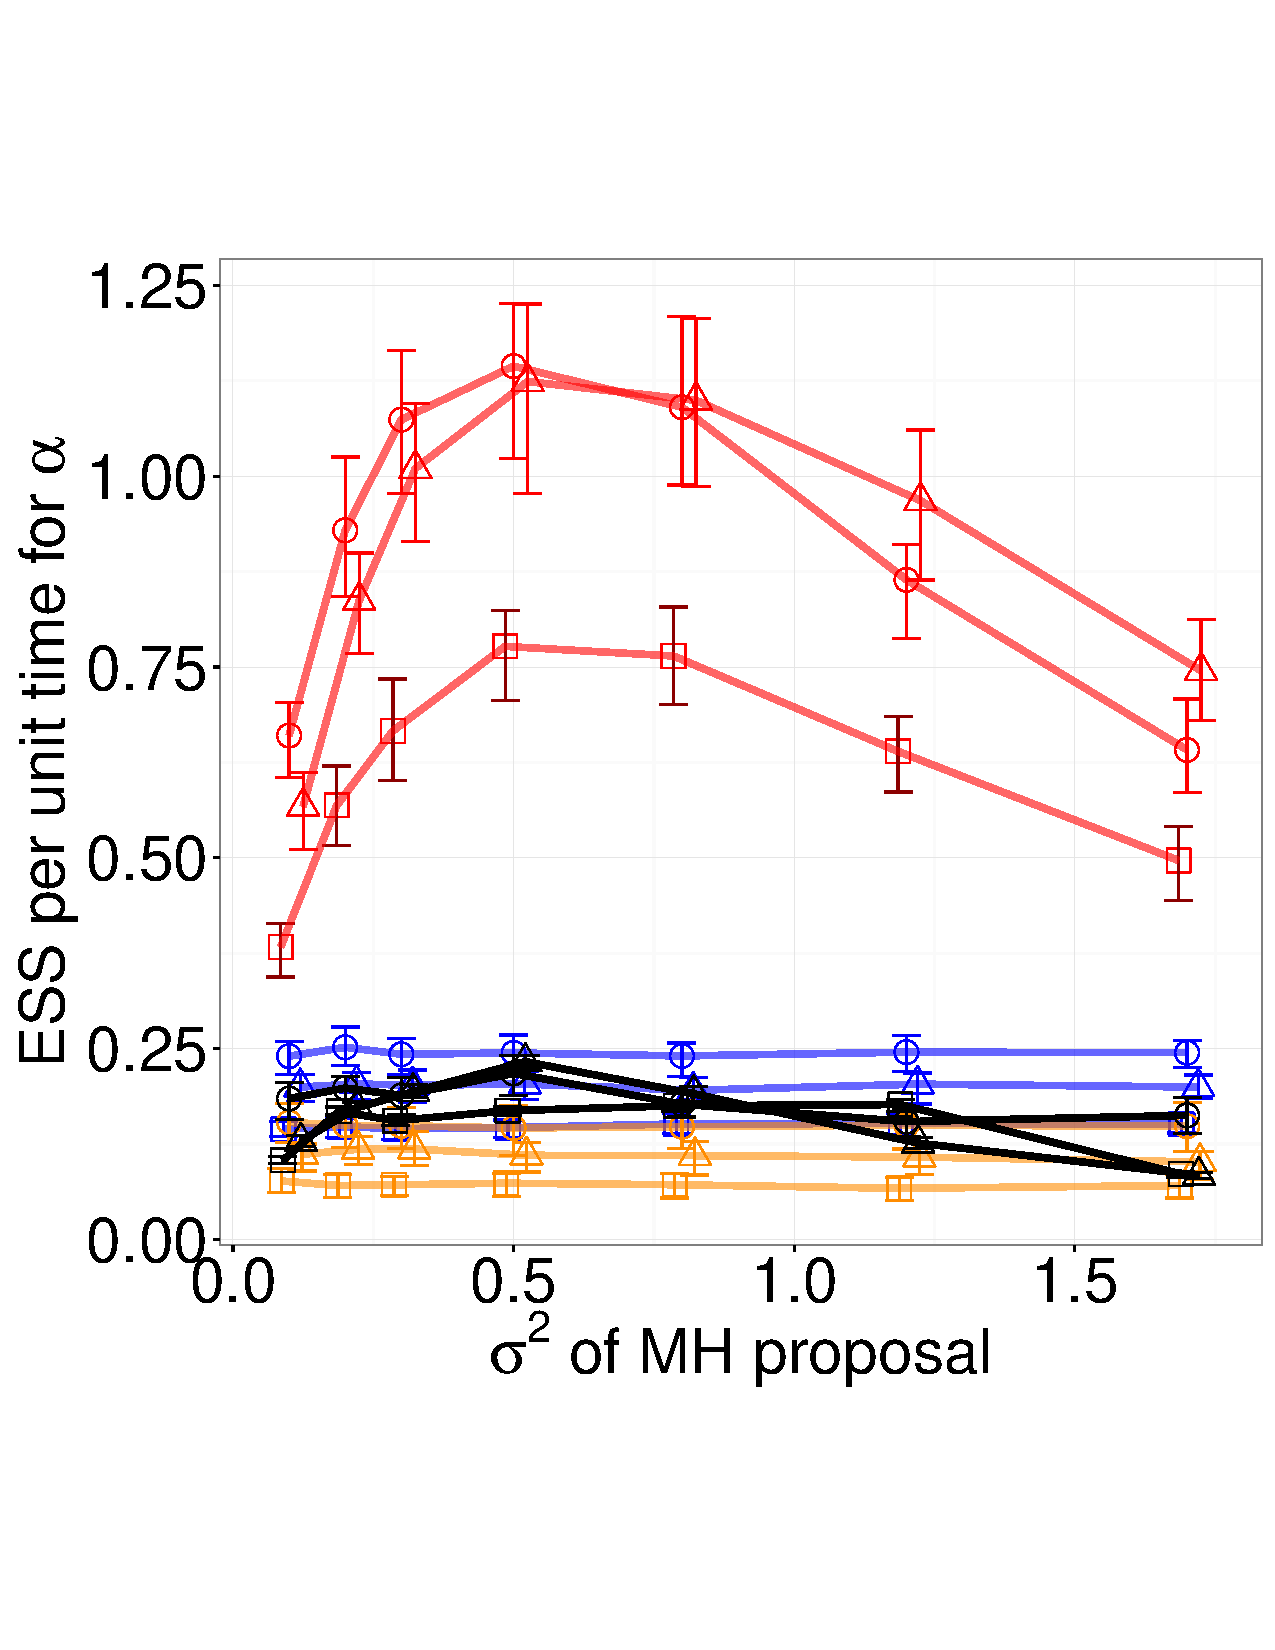
\includegraphics [width=0.90\textwidth, angle=0]{figs/exp_10_alpha.pdf}
      \end{minipage}
  \begin{minipage}[hp]{0.45\linewidth}
  \centering
    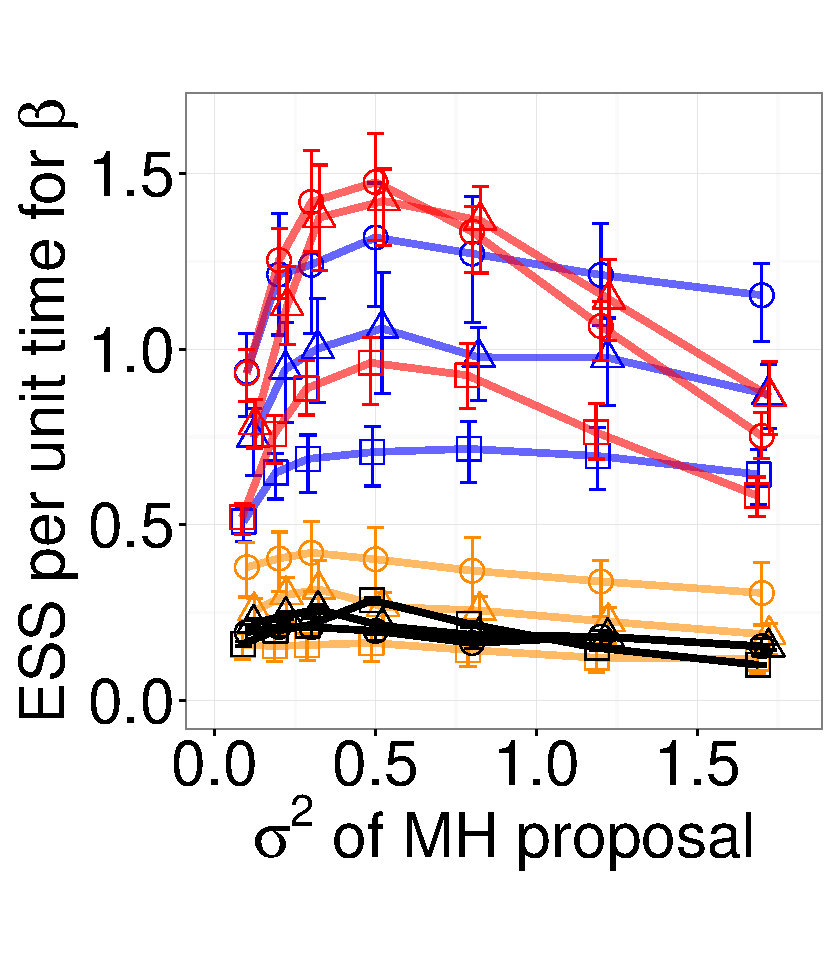
\includegraphics [width=0.90\textwidth, angle=0]{figs/exp_10_beta.pdf}
    \vspace{-0 in}
  \end{minipage}
    \caption{ESS/sec for exp model (dim 10). The left is for $\alpha$, and the right is for $\beta$.}
     \label{fig:ESS_EXP_D10}
  \end{figure}
  Figures~\ref{fig:ESS_EXP_D3} and~\ref{fig:ESS_EXP_D10} plot the ESS 
  per unit time for the parameters $\alpha$ (left) and $\beta$ (right) for the
  case of $3$ and $10$ states (we include results for $5$ states in the 
  supplementary material, the conclusions are the same). 
  %as we change the variance of the
  %proposal kernel, for different methods and different scaling parameters.
  %($\kappa =
%1.5, 2, 3$) and dimensions($p = 3, 5, 10$).
%, where   $k = 1.5$,  $\Omega(\theta, \theta^*) = k \max(\max A(\theta), \max A(\theta^*))$. 
%For particle MCMC, the number of particles can be $5, 10 , 20$. 
  Blue lines are the Gibbs sampler, orange lines are simple MH, red lines 
are the symmetrized MH and black lines are particle MCMC. 
(\vinayak{Do we have these (dots,triangles, squares?)}
{\color{red} Lines with dots correspond to $k = 1.5$. 
Lines with triangle correspond to $k = 2$. 
Lines with squares correspond to $k = 3$.  )
The black dot dash lines correspond to $N  = 5$. 
The dash black lines correspond to $N  = 10$. 
The solid black lines correspond to $N  = 20$. $N$ is the number of particles. 
For $k=$ $2$ or $3$, $\Omega(\theta, \theta^*) = 
\frac{k}{2} (\max A(\theta) + \max A(\theta^*))$. }

We see that our symmetrized MH algorithm is significantly more efficient 
than the baselines over a wide range of choices of the proposal distribution 
(including the natural choice of $1$).
Among the three setting of our algorithm, the simple additive setting
$\Omega = (\Omega_{old} + \Omega_{new})$ (shown as the curve with triangles) 
does best, though it is not significantly better than 
$\Omega = 2(\Omega_{old} + \Omega_{new})$ (shown with circles).
$\Omega = 1.5 \max(\Omega_{old}, \Omega_{new})$ (plotted with circles) does 
worse than both additive choices.
Among the baselines, simple Gibbs sampling \vinayak{what are the different curves?}
does better than \naive\ Metropolis-Hastings\vinayak{what are the different curves?}, 
suggesting that the dependency of the 
uniformization on the MJP parameters can significantly slow down mixing.
Particle MCMC has the worst performance for this task.

  \begin{figure}%[b]    
  \centering
  \begin{minipage}[hp]{0.24\linewidth}
  \centering
    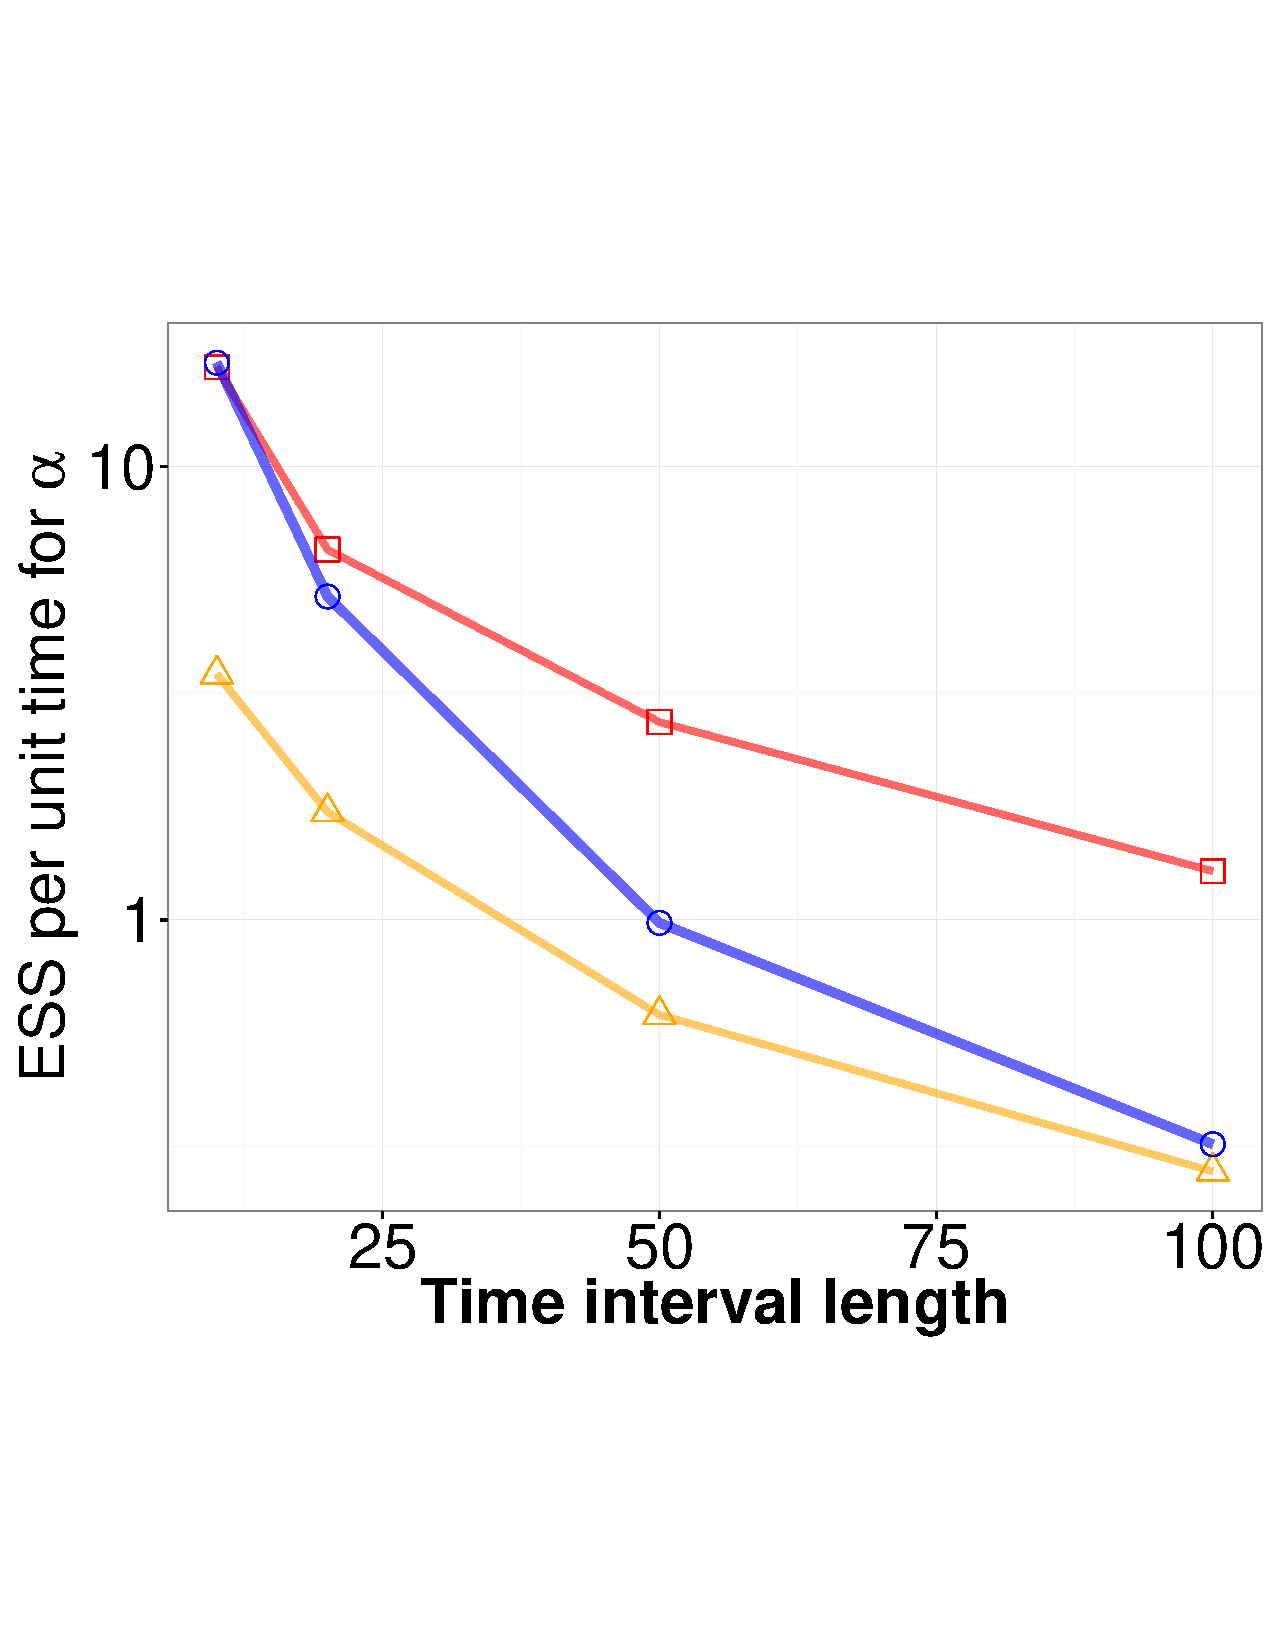
\includegraphics [width=0.99\textwidth, angle=0]{figs/ESS_vs_t_alpha_fixobservation.pdf}
    \end{minipage}
  \begin{minipage}[hp]{0.24\linewidth}
  \centering
    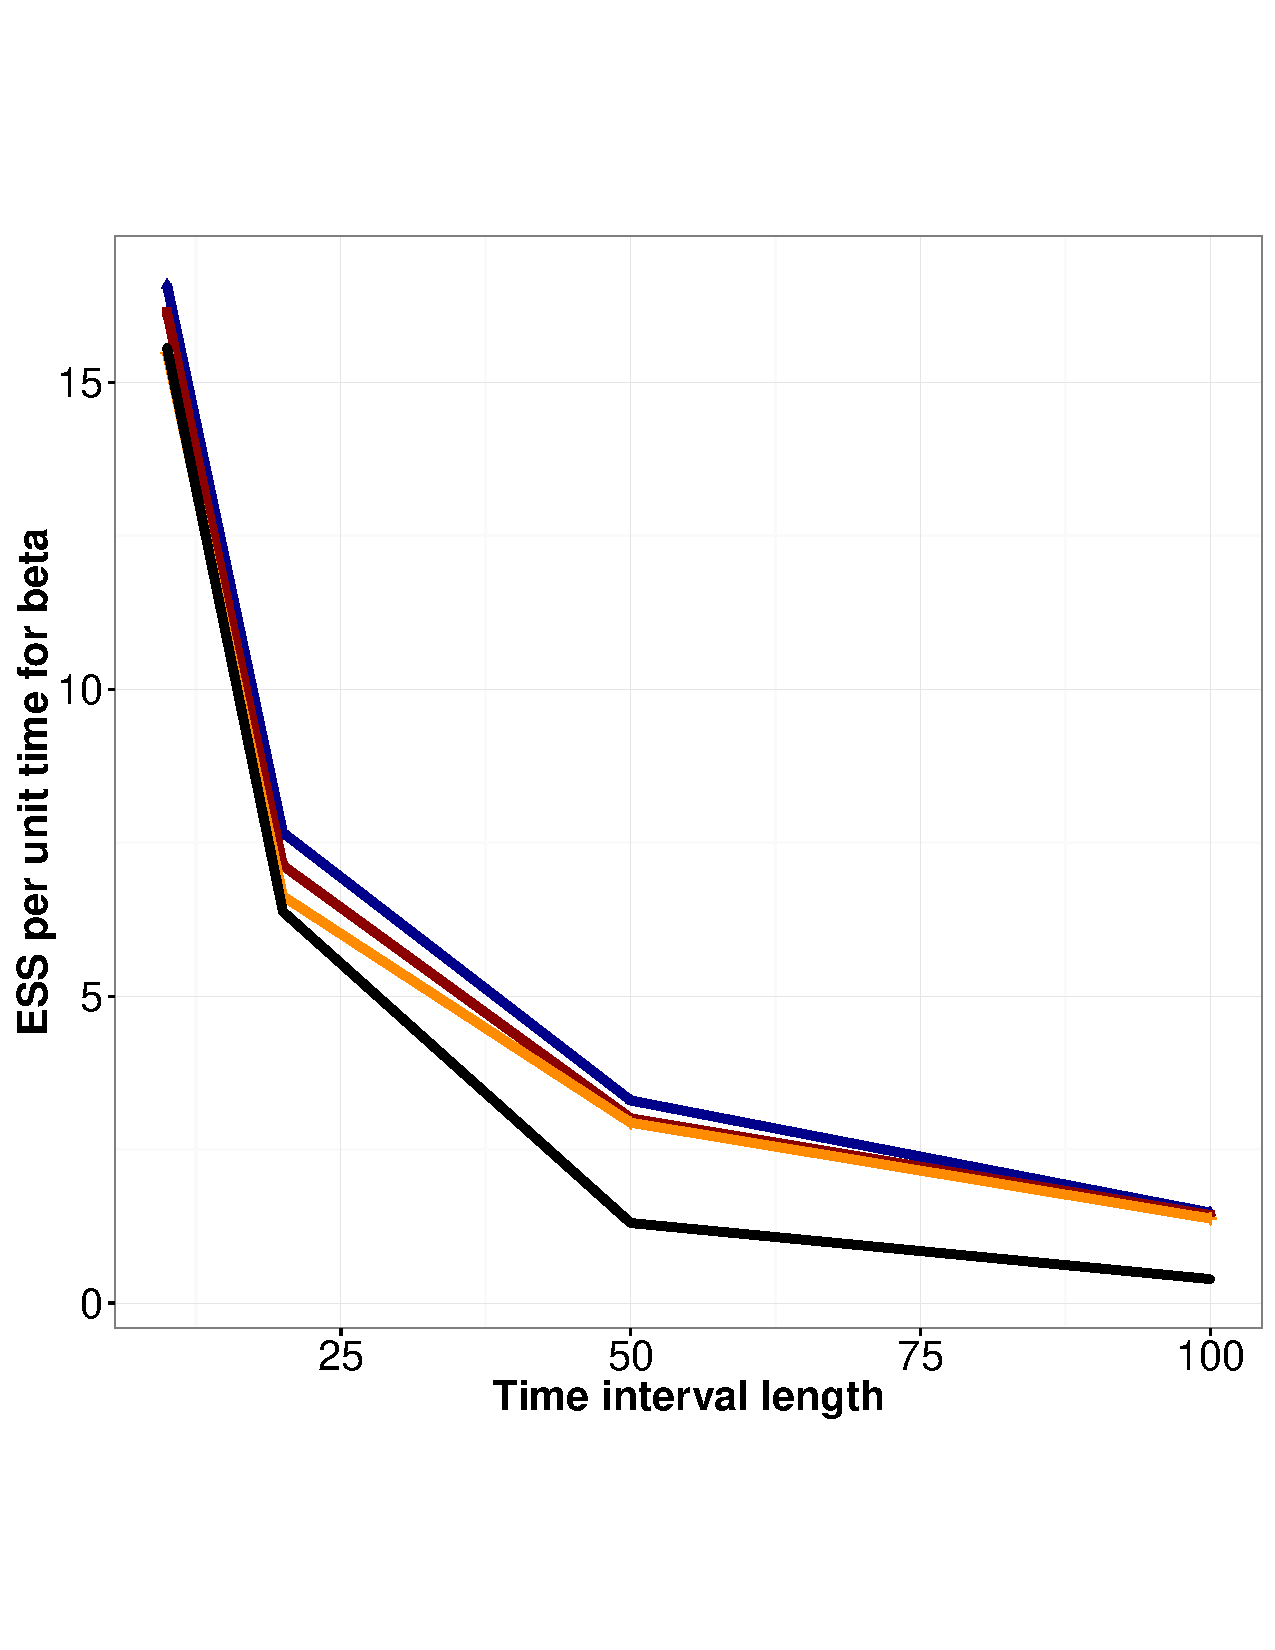
\includegraphics [width=0.99\textwidth, angle=0]{figs/ESS_vs_t_beta_fixobservation.pdf}
%    \vspace{-0.3in}
  \end{minipage}
    %\label{fig:TSS_fix}
  \begin{minipage}[hp]{0.24\linewidth}
  \centering
    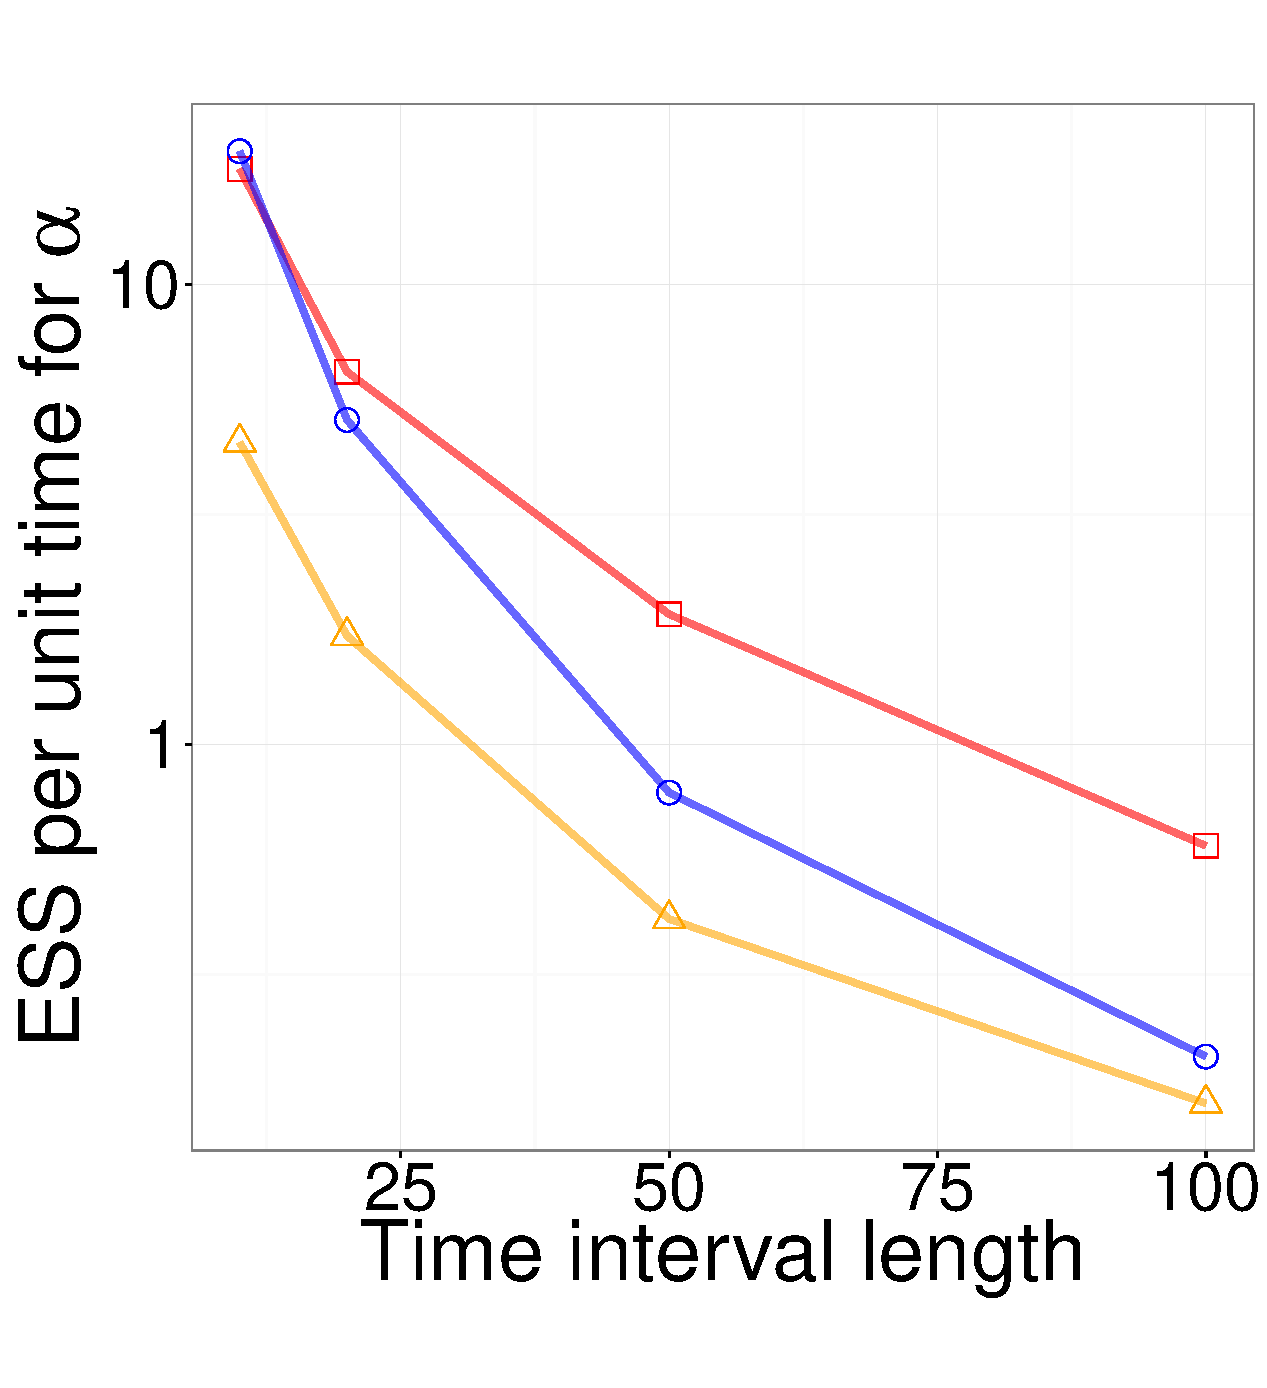
\includegraphics [width=0.99\textwidth, angle=0]{figs/ESS_vs_t_alpha.pdf}
      \end{minipage}
  \begin{minipage}[hp]{0.24\linewidth}
  \centering
    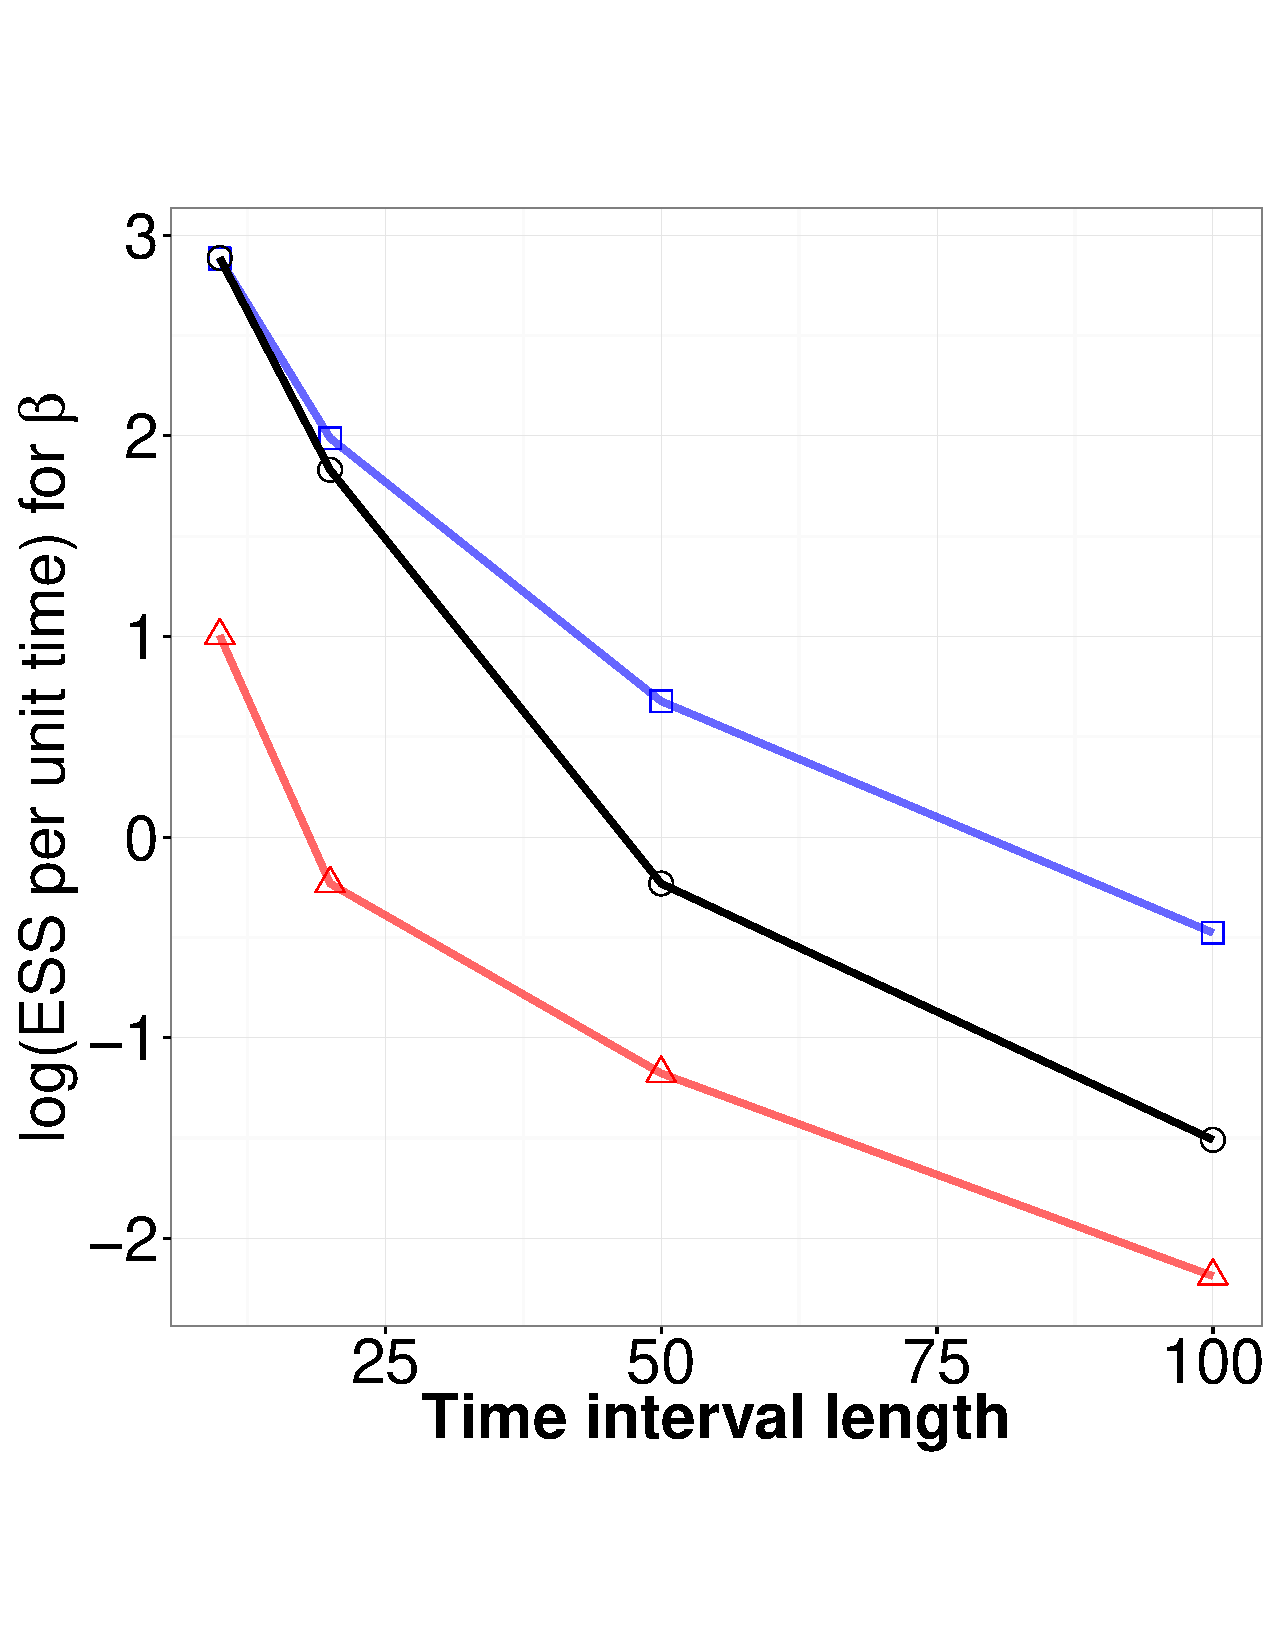
\includegraphics [width=0.99\textwidth, angle=0]{figs/ESS_vs_t_beta.pdf}
  \end{minipage}
    \vspace{-0.3in}
%    \caption{Time Interval vs. ESS / sec}
    \caption{Time Interval vs. ESS / sec (Number of observations is fixed)}
     \label{fig:TSS}
  \end{figure}
In Figure~\ref{fig:TSS_fix}, we plot ESS per unit time as the observation 
interval increases. 
%We generate different observations on different time intervals. 
%Our observation process was a Gaussian distribution with mean equal to the 
%current state and variance equal to $1$. 
As before there are $19$ observations uniformly located over a time interval
$(0,\cT)$, now $\cT$ can be $10, 20, 50, 100$. We consider the three-state 
MJP, and compare our symmetrized algorithm (with $\kappa$ set to $1$) with
the Gibbs sampler. 
While the Gibbs sampler (the black line) performs well for the smallest value
of $\cT$, its performance is considerably worse for longer time-intervals.
This is because longer time interval result in stronger coupling between MJP
path and parameter, affecting mixing. The effect of this coupling is much milder
if we integrate out the MJP trajectory.

In Figure~\ref{fig:TSS}, we plot results from a similar experiment. Now,
instead of keeping the number of measurements fixed as we increase the observation
interval, we keep the observation rate fixed at one observation every unit
interval of time, so that longer observation intervals have larger number of 
observations. The results are similar to the previous case: Gibbs sampling
performs well for small observation intervals, with performance degrading
sharply for larger observation intervals. These two experiments illustrate the 
usefulness of our idea of integrating out the MJP path while carrying out
parameter inference.

\subsection{An Immigration model with finite capacity}\label{sec:immig}~
 Our next experiment considers an M/M/N/N queue (figure~\ref{q_model}). This is a stochastic process 
whose state space is the set $\{0, 1, 2, 3, \cdots, N - 1\}$ with elements
giving the number of customers/jobs in a system or individuals in a population. 
Arrivals follow a rate-$\alpha$ Poisson process, moving the process from state 
$i$ to $i+1$ for $i<N$. The system has a capacity of $N$, so any arrivals when 
the current state is $N$ are discarded.  Service times or deaths are 
exponentially distributed, with a rate that is now state-dependent:
the system moves from $i$ to $i - 1$ with rate $i\beta$. 
%There are $N$ servers, which serve from the front of the queue. 
%If there are less than $N$ jobs, some of the servers will be idle. 
%Only $N$ customers can queue at any one time. 
%Any further arrivals to the queue are considered ''lost''. 

We follow the same procedure as the previous experiment:
for $(\alpha_0,\alpha_1,\beta_0,\beta_1)$ equal to $(3,2,5,2)$,
we place Gamma$(\alpha_0,\alpha_1)$, and Gamma$(\beta_0, \beta_1)$ priors on 
$\alpha$, $\beta$. These prior distributions were used to sample transition 
matrices $A$, and generate MJP trajectories, which we observe at integer-valued
times according to a Gaussian observation process.
We consider three settings: $3, 5$ and $10$ states, with results from $5$ 
steps included in the supplementary material. 

  \begin{figure}
  \centering
  \begin{minipage}[hp]{0.6\linewidth}%0.45
  \centering
    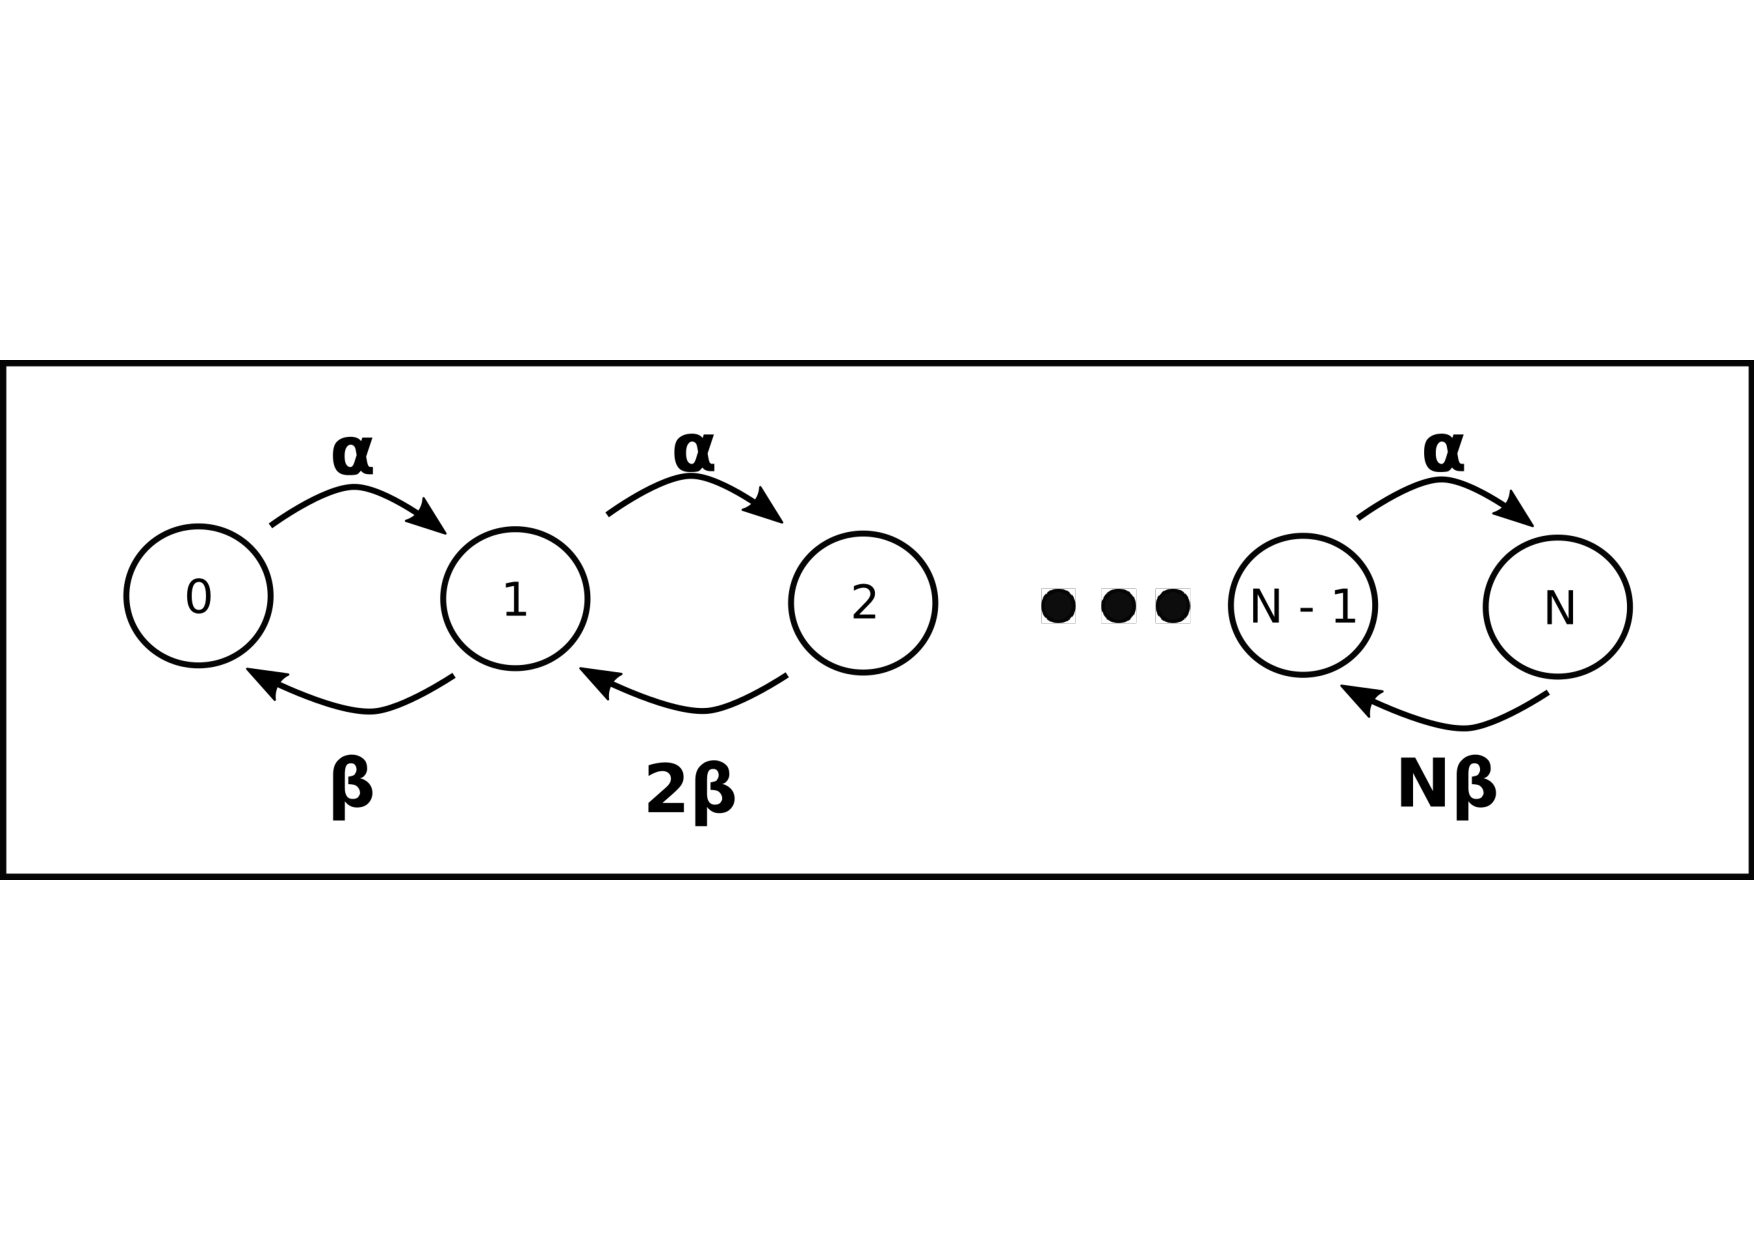
\includegraphics [width=1\textwidth, angle=0]{figs/queue_model.pdf}%0.70
      \end{minipage}
    \caption{queuing model}
	\label{q_model}
  \end{figure}
  %\subsection{Experiments}
  In Figure~\ref{fig:ESS_Q_D3}, Figure~\ref{fig:ESS_Q_D5}, Figure~\ref{fig:ESS_Q_D10} we plot the ESS per unit time for the parameters $\alpha$ (left) and $\beta$ (right) as we change the variance of the
  proposal kernel per run, for different methods and different scaling parameters k($k = 1.5, 2, 3$) and different dimensions($p = 3, 5, 10$), where   $k = 1.5$,  $\Omega(\theta, \theta^*) = k \max(\max A(\theta), \max A(\theta^*))$. Blue lines are for Gibbs sampler. Red lines are for improved MH. Orange lines are for naive MH. Black lines are for particle MCMC. Lines with dots correspond to $k = 1.5$. Lines with triangle correspond to $k = 2$. Lines with squares correspond to $k = 3$. For $k=$ $2$ or $3$, $\Omega(\theta, \theta^*) = \frac{k}{2} (\max A(\theta) + \max A(\theta^*))$. We see that the improved MH algorithm is more efficient i	n these cases with respect to the overall ESS per unit time. We also see that increase the scaling parameter will decrease the efficiency of the improved MH algorithm respect to overall ESS per unit time, when $k > 2$. If we set $\Omega = 1.5 \max(\Omega_{old}, \Omega_{new})$, the performance of the improved MH will not be as good as the case we set $\Omega = 2(\Omega_{old} + \Omega_{new})$ when the proposal log variance is large.\\

% Figure~\ref{fig:hist} shows posterior distributions for 
% $P(\theta | X)$(red), $P(\theta | S, T, X)$(green), $P(\theta | W, X)$(blue). 
% We run $10000$ iterations. The first $5000$ are treated as burn in period. 
% We fix $V_{5000}, W_{5000}$ and then sample $\theta$ from 
% $P(\theta | V_{5000}, W_{5000}, X)$ and sample $\theta$ from 
% $P(\theta | W_{5000}, X)$. We keep updating $S$ and $T$ for sampling from 
% $P(\theta | X)$. We sample another $5000$ $\theta$s to draw the histograms. 
% We can find that $P(\theta | S, T, X)$ and $P(\theta | W, X)$ are both very 
% concentrated which implies the coupling.
  \begin{figure}%[b]
  \centering
  \begin{minipage}[hp]{0.45\linewidth}
  \centering
    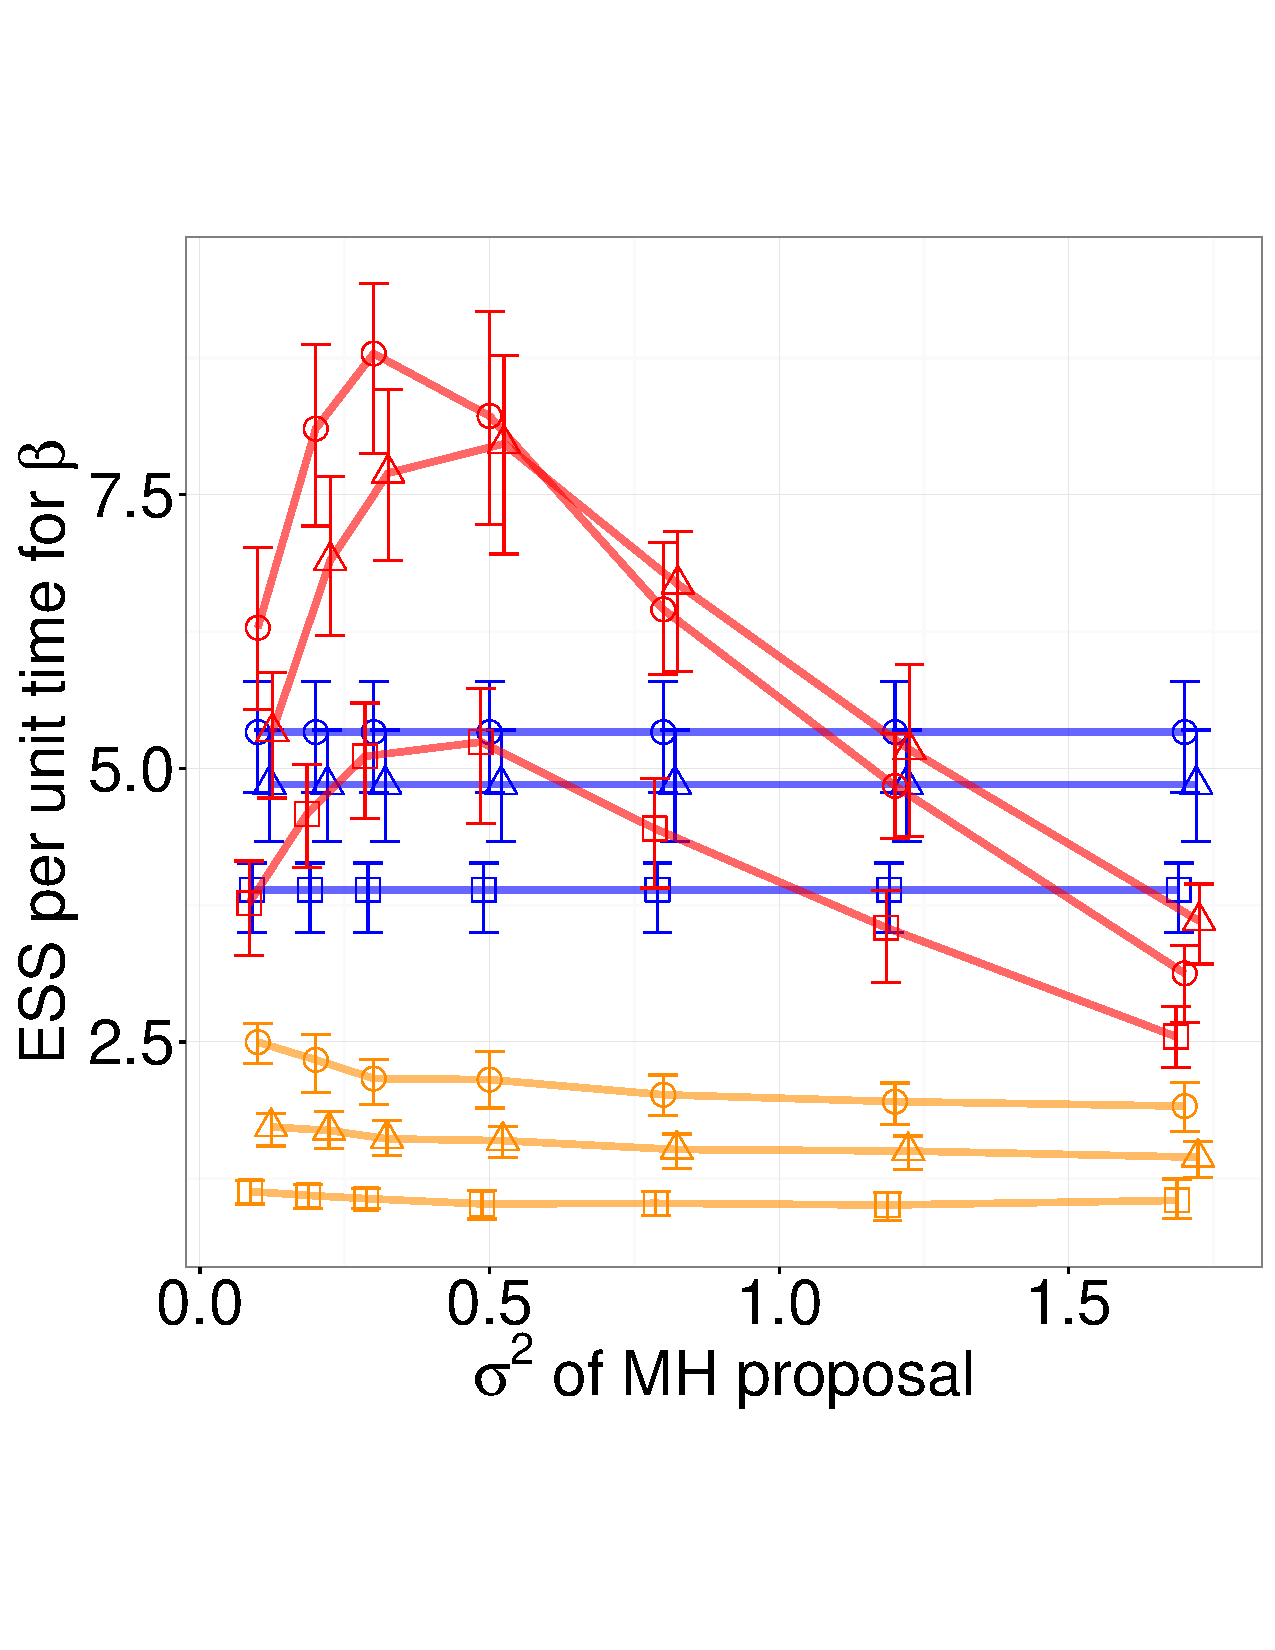
\includegraphics [width=0.90\textwidth, angle=0]{figs/q_3_alpha.pdf}
      \end{minipage}
  \begin{minipage}[hp]{0.45\linewidth}
  \centering
    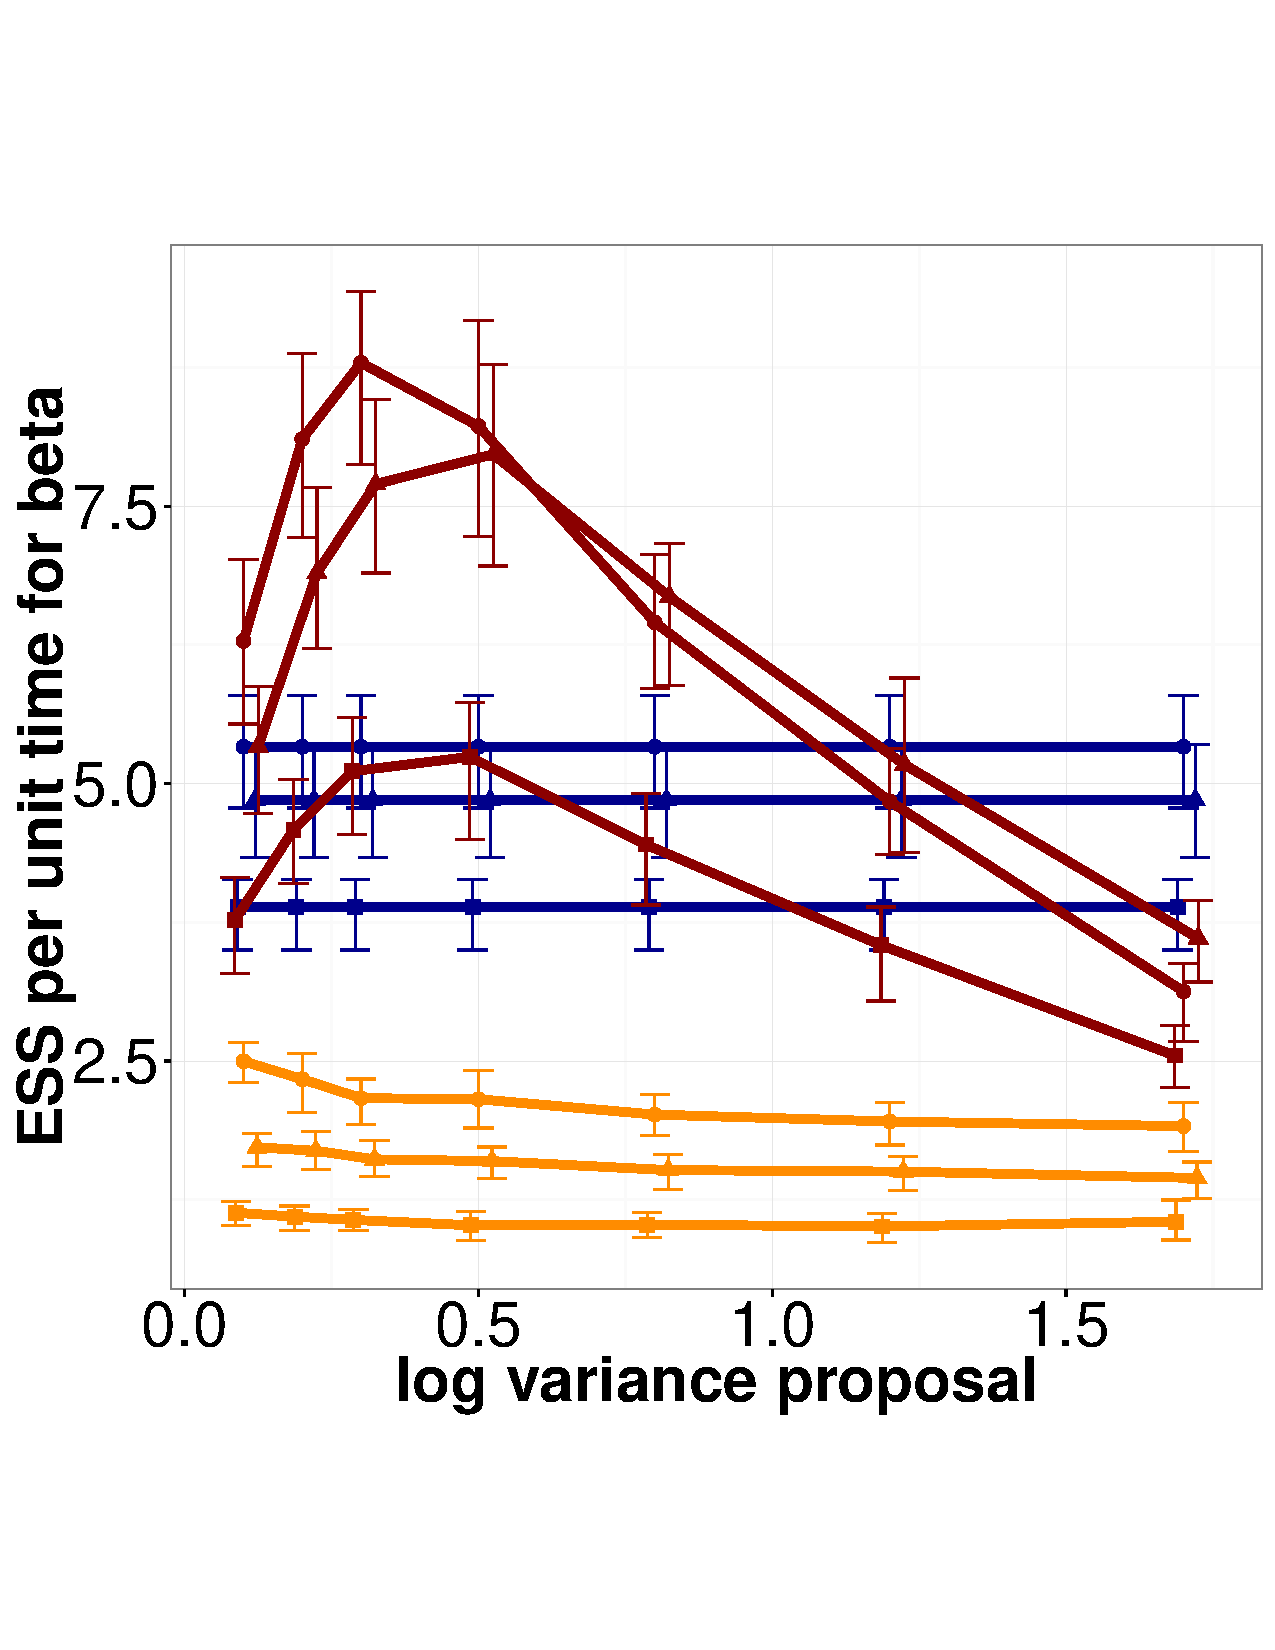
\includegraphics [width=0.90\textwidth, angle=0]{figs/q_3_beta.pdf}
    \vspace{-0 in}
     \label{fig:ESS_Q_D3}
  \end{minipage}
    \caption{ESS/sec for Immigration model (dim 3).The left is for $\alpha$, and the right is for $\beta$.}
  \end{figure}

  \begin{figure}%[b]
  \centering
  \begin{minipage}[!hp]{0.45\linewidth}
  \centering
    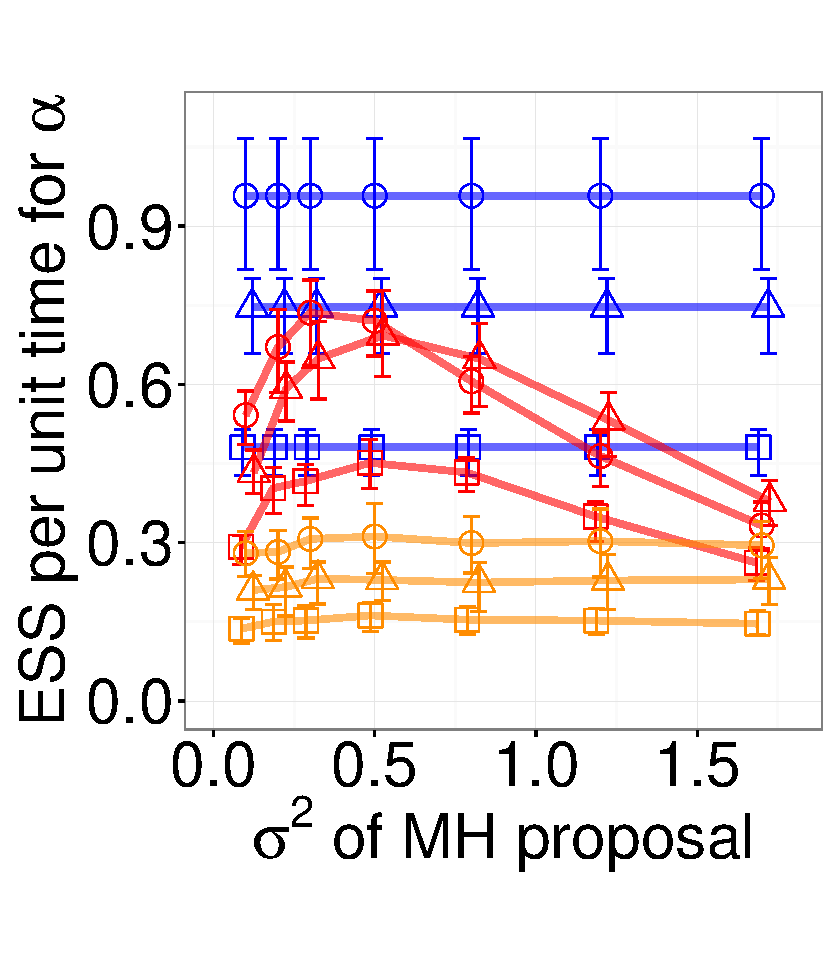
\includegraphics [width=0.90\textwidth, angle=0]{figs/q_10_alpha.pdf}
      \end{minipage}
  \begin{minipage}[hp]{0.45\linewidth}
  \centering
    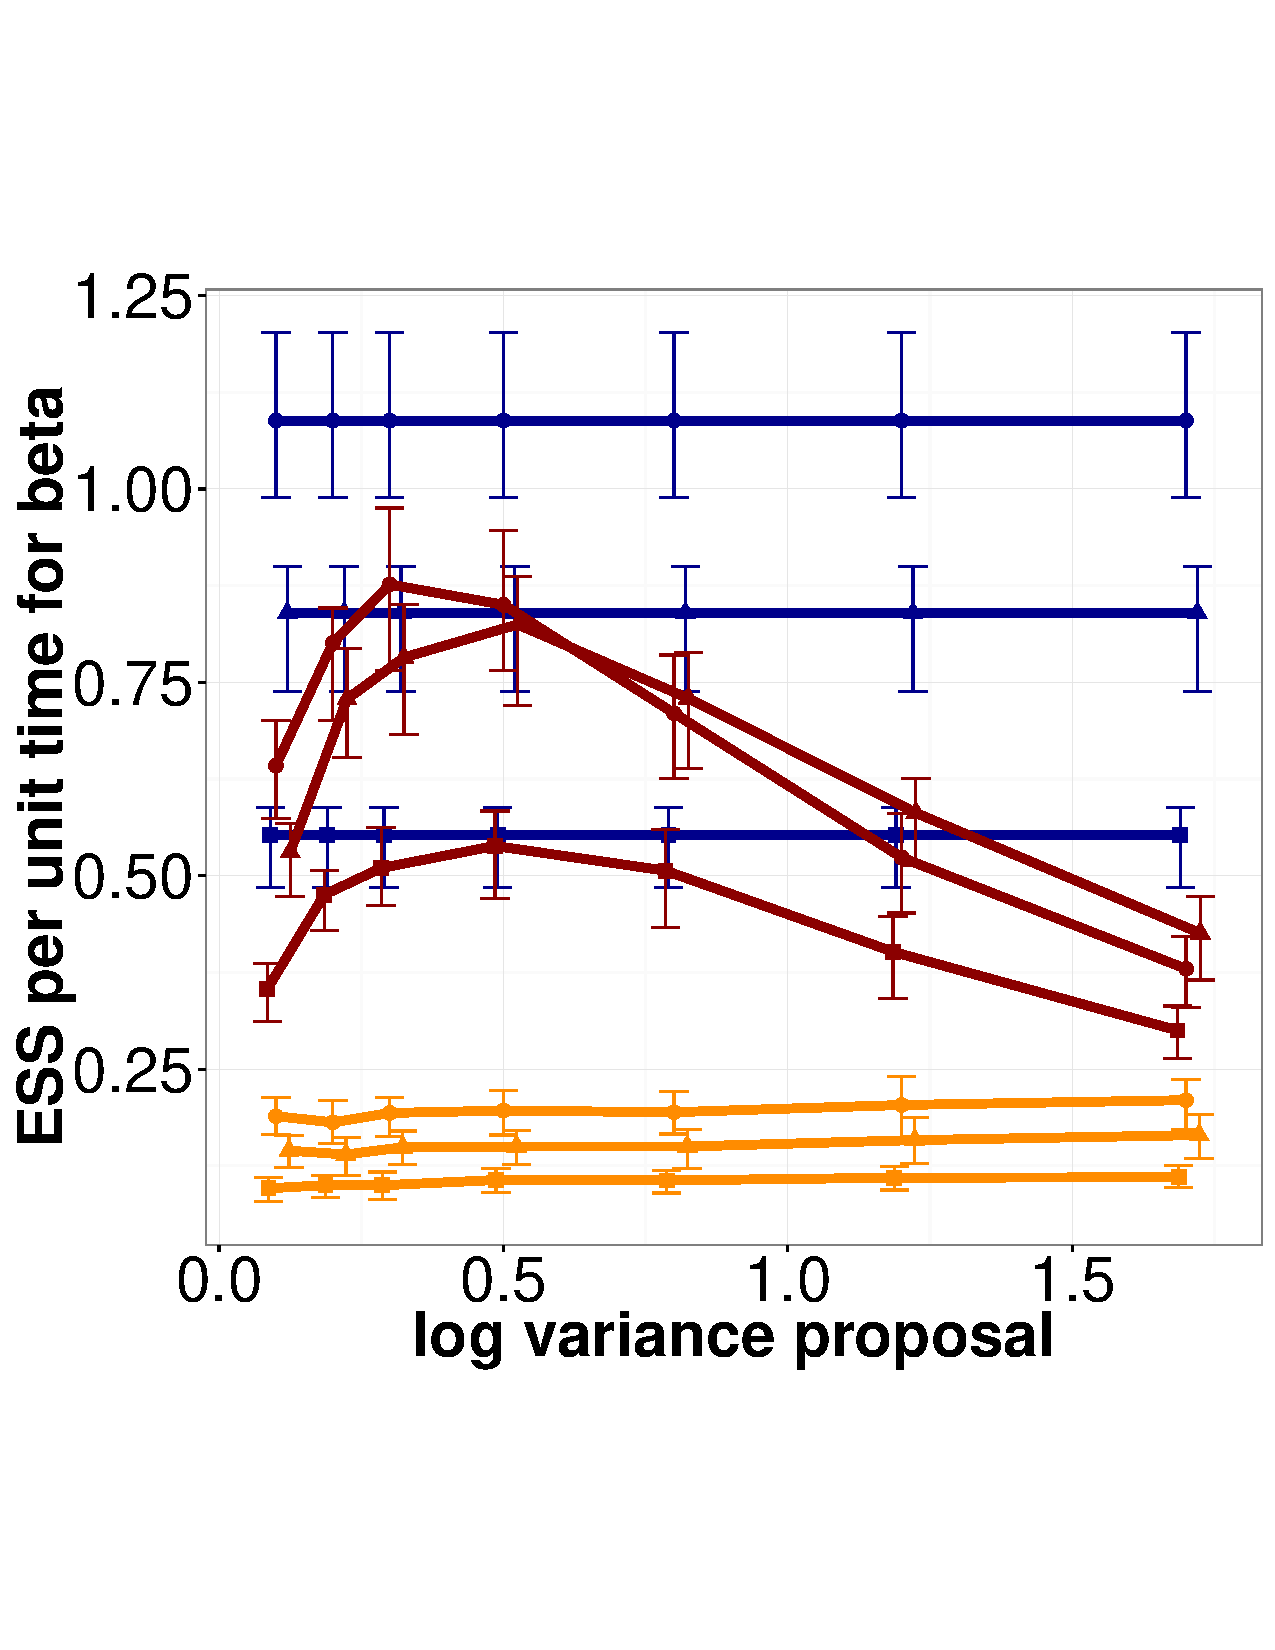
\includegraphics [width=0.90\textwidth, angle=0]{figs/q_10_beta.pdf}
    \vspace{-0 in}
     \label{fig:ESS_Q_D10}
  \end{minipage}
    \caption{ESS/sec for Immigration model (dim 10).The left is for $\alpha$, and the right is for $\beta$.}
  \end{figure}
% \begin{figure}%[b]
% \begin{minipage}[hp]{0.45\linewidth}
% \centering
%   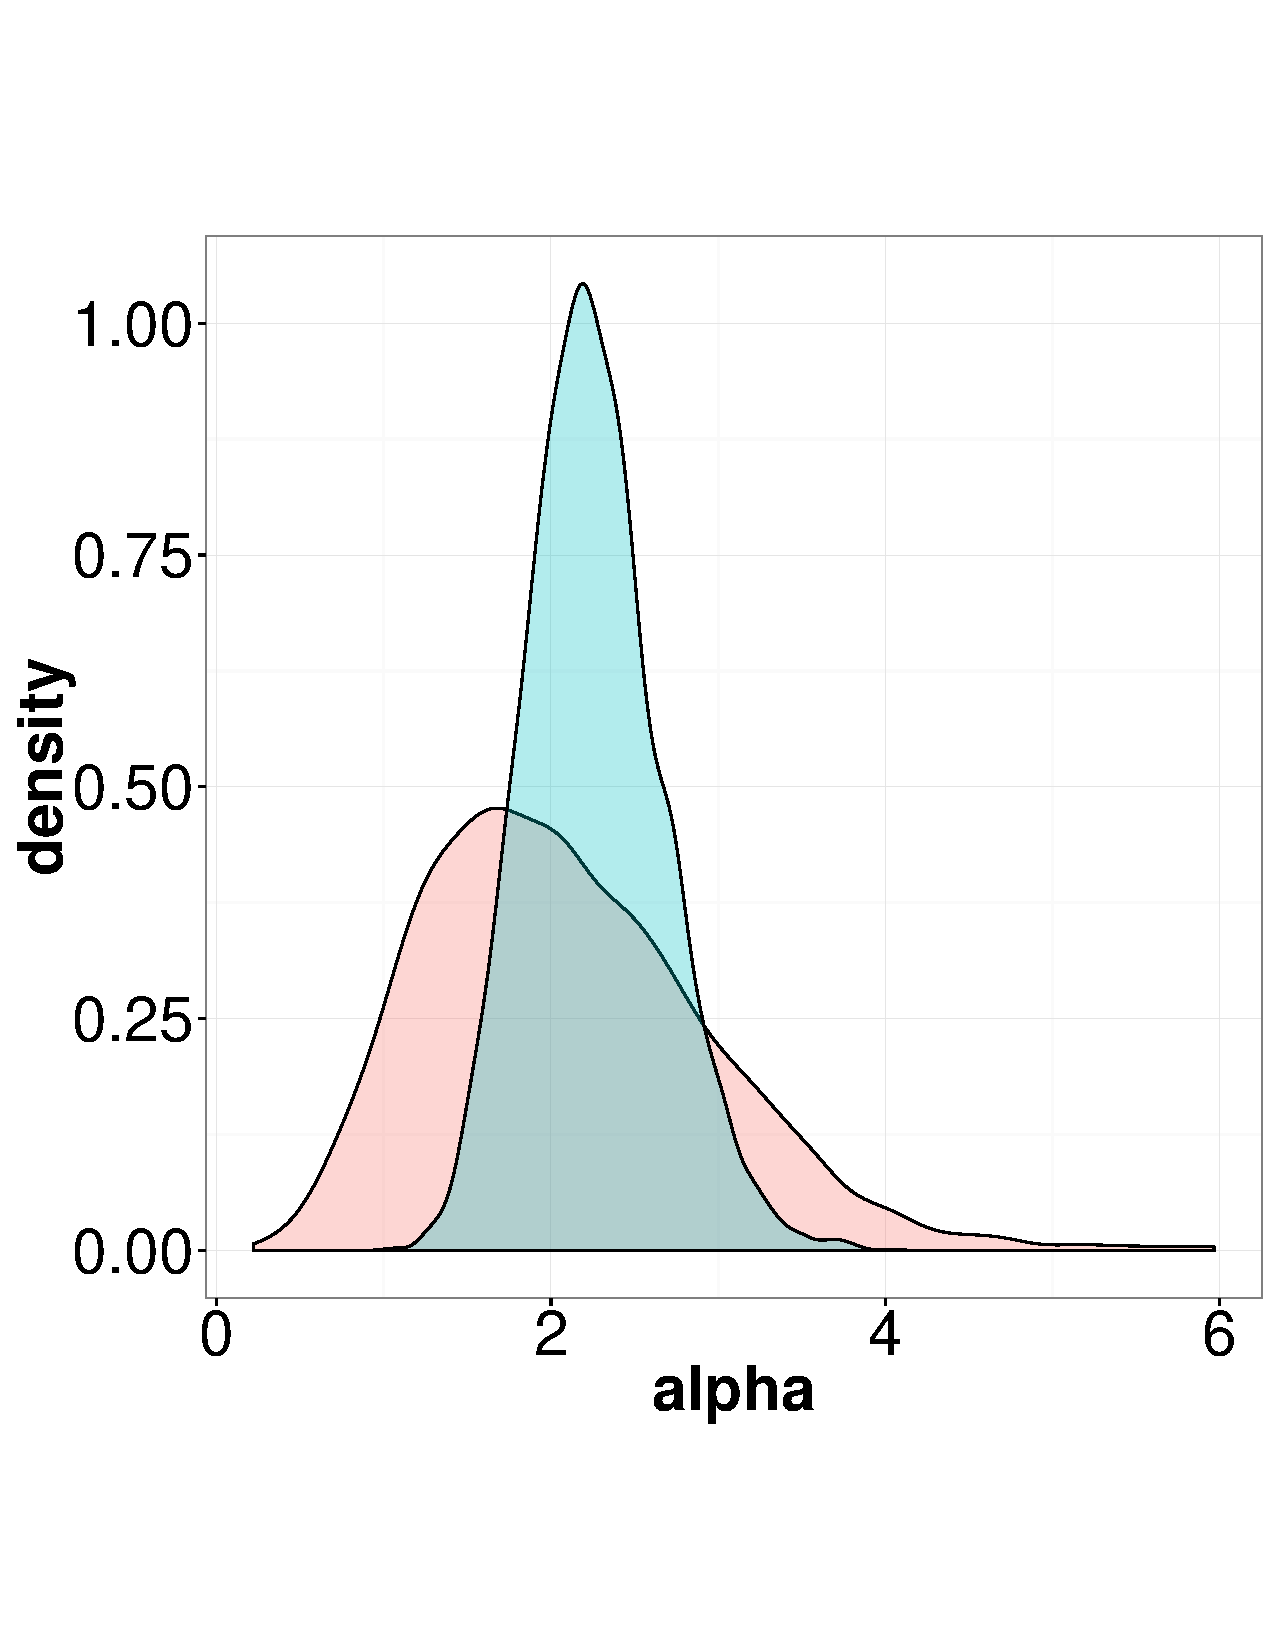
\includegraphics [width=0.90\textwidth, angle=0]{figs/dist_alpha.pdf}
%   \vspace{-0 in}
% \end{minipage}
% \begin{minipage}[!hp]{0.45\linewidth}
% \centering
%   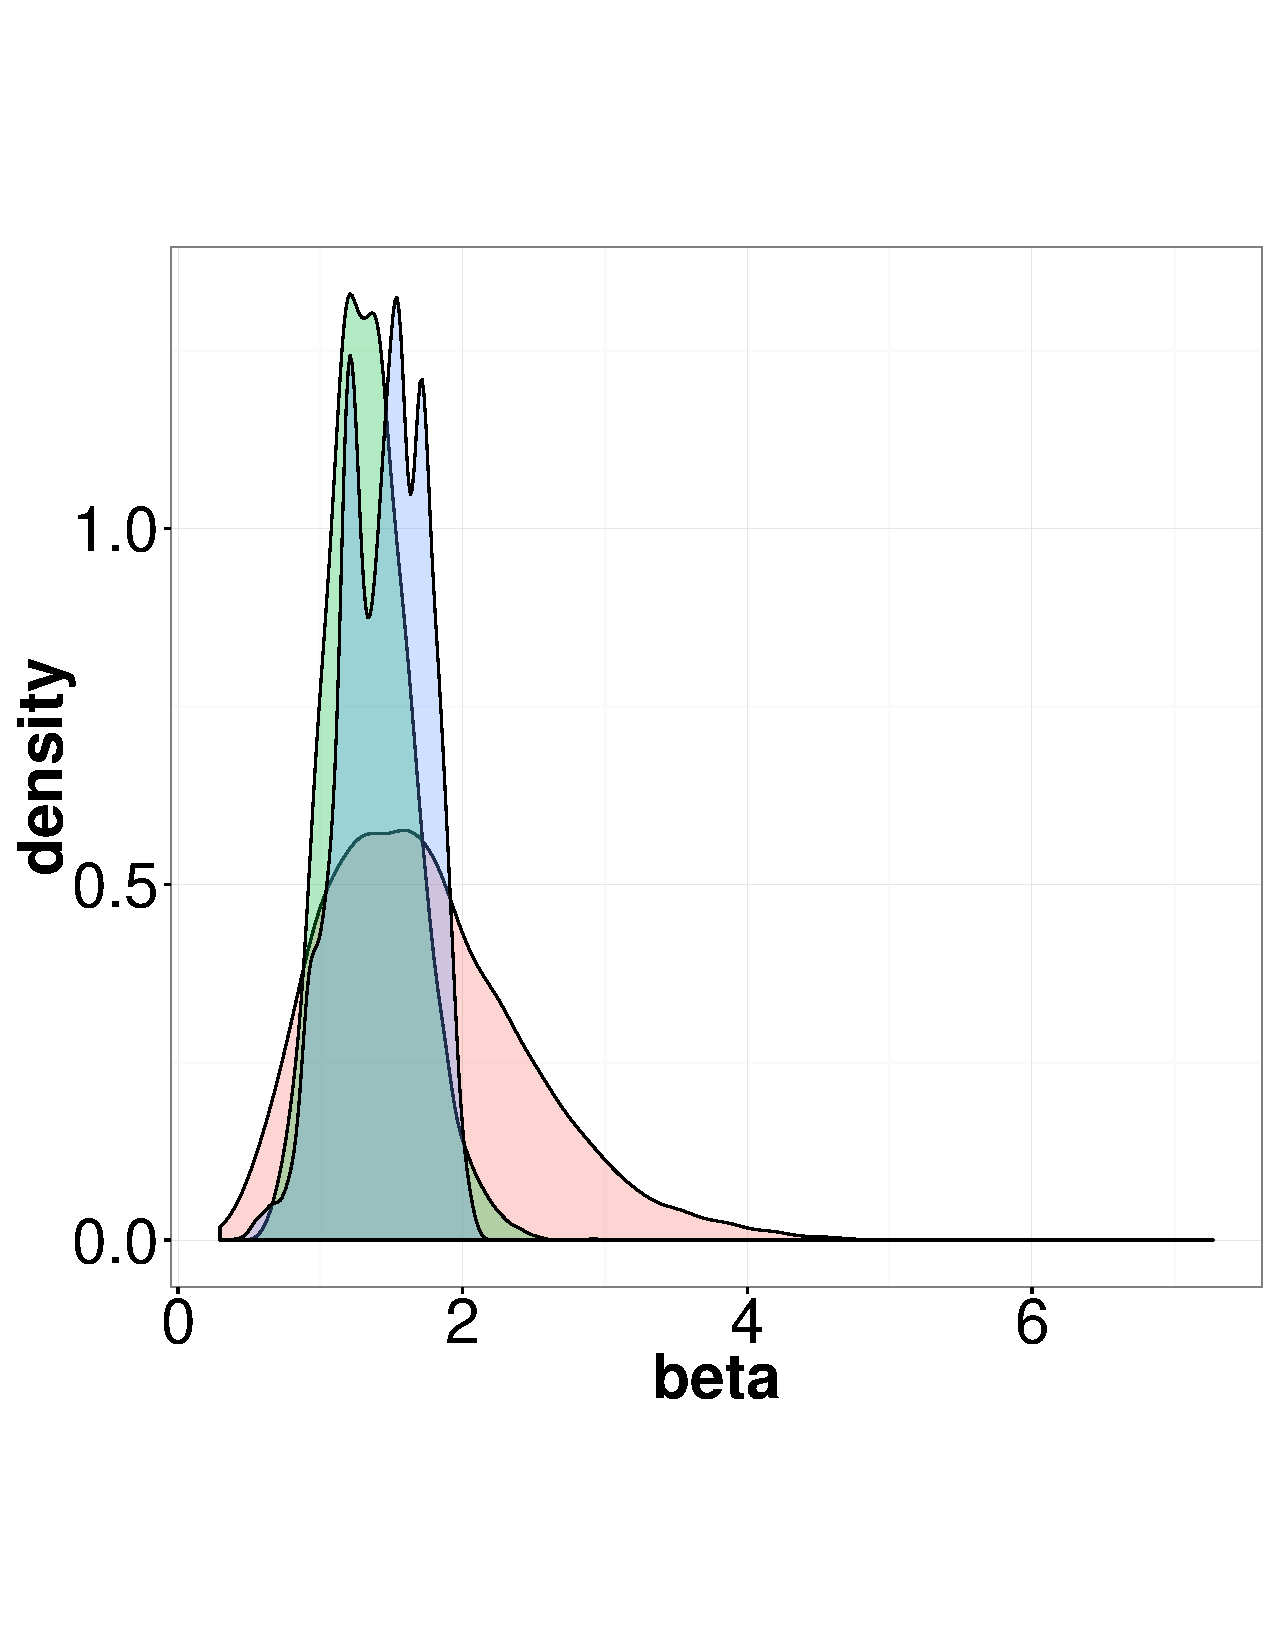
\includegraphics [width=0.90\textwidth, angle=0]{figs/dist_beta.pdf}
%   \vspace{-0 in}
% \end{minipage}
%   \caption{density.The left is for $\alpha$, and the right is for $\beta$.}
%    \label{fig:dist}
% \end{figure}


  \subsection{The Jukes and Cantor (JC69) model}~
  \begin{figure}%[H]
  \centering
  \begin{minipage}[!hp]{0.45\linewidth}
  \centering
    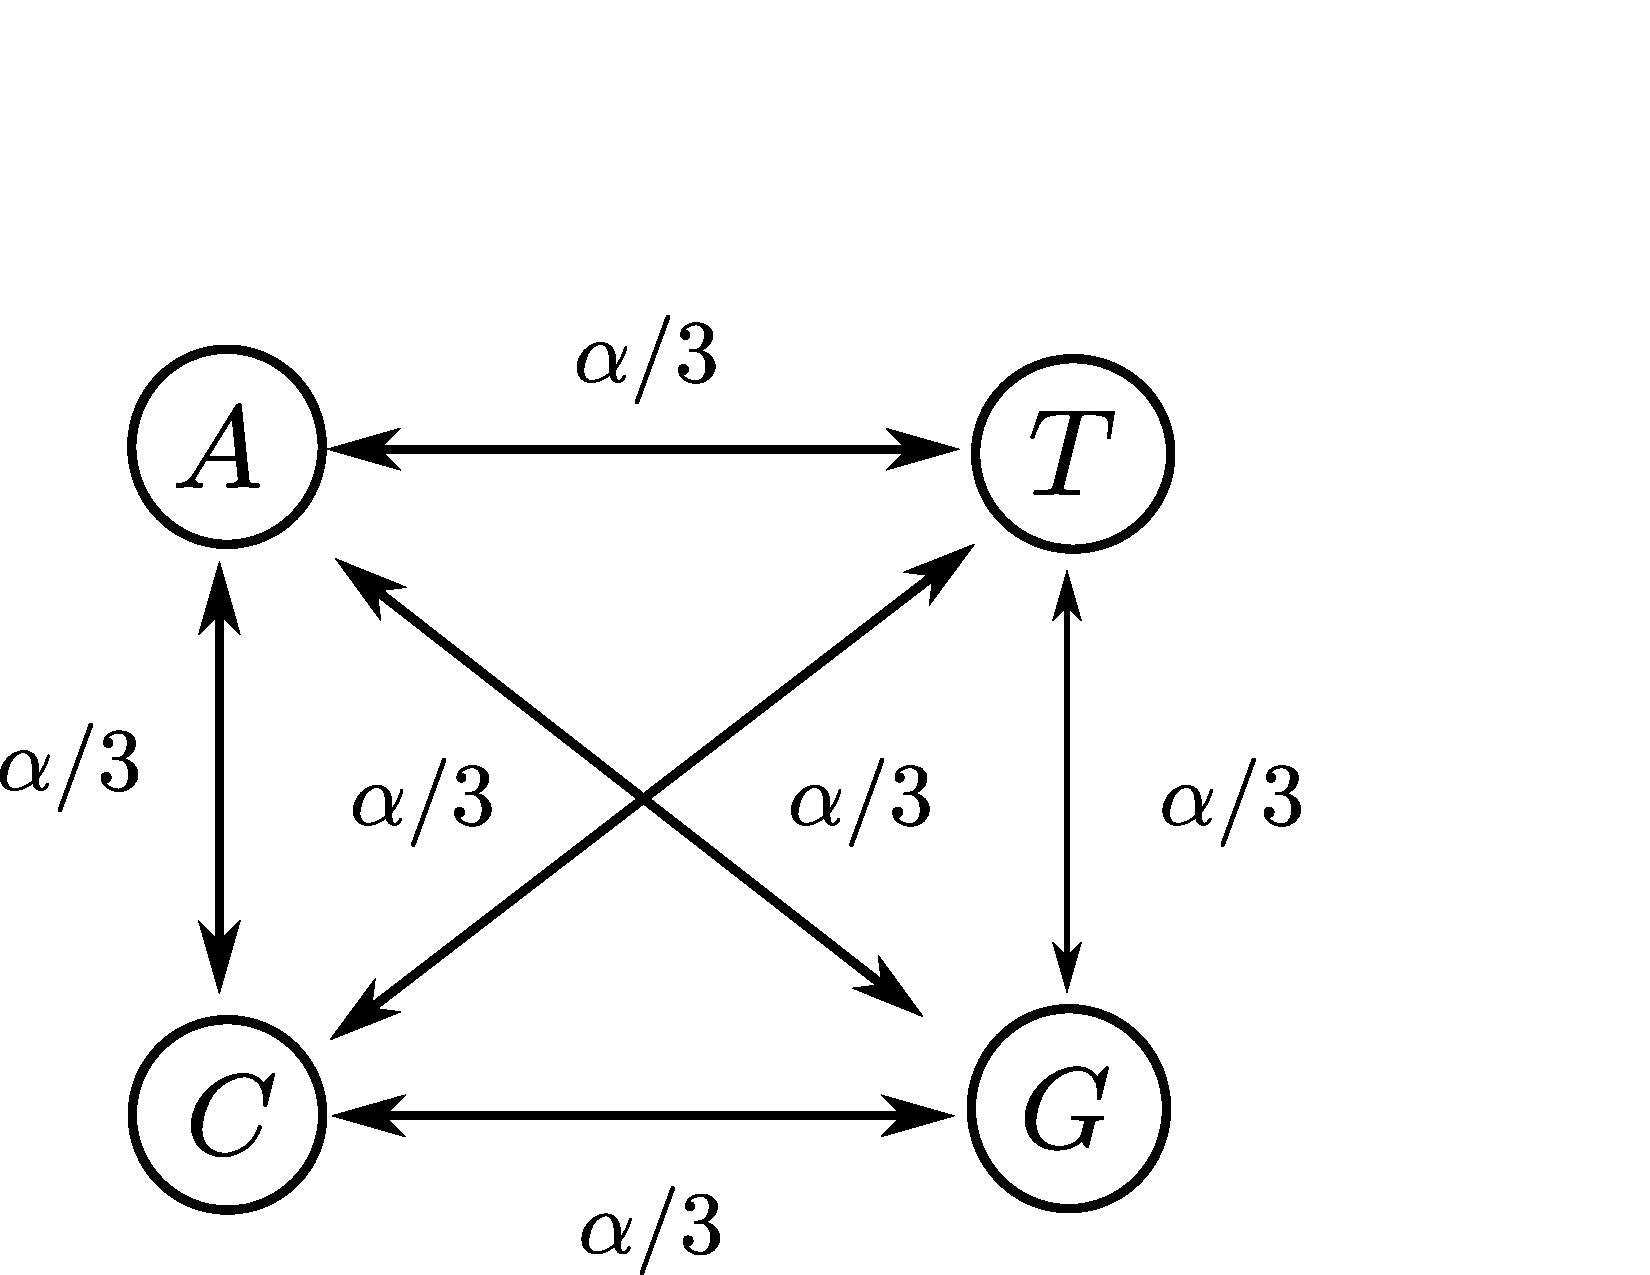
\includegraphics [width=0.90\textwidth, angle=0]{figs/jc_model.pdf}
    \caption{JC69 model}
	\label{jc_model}
  \end{minipage}
  \begin{minipage}[!hp]{0.45\linewidth}
  \centering
    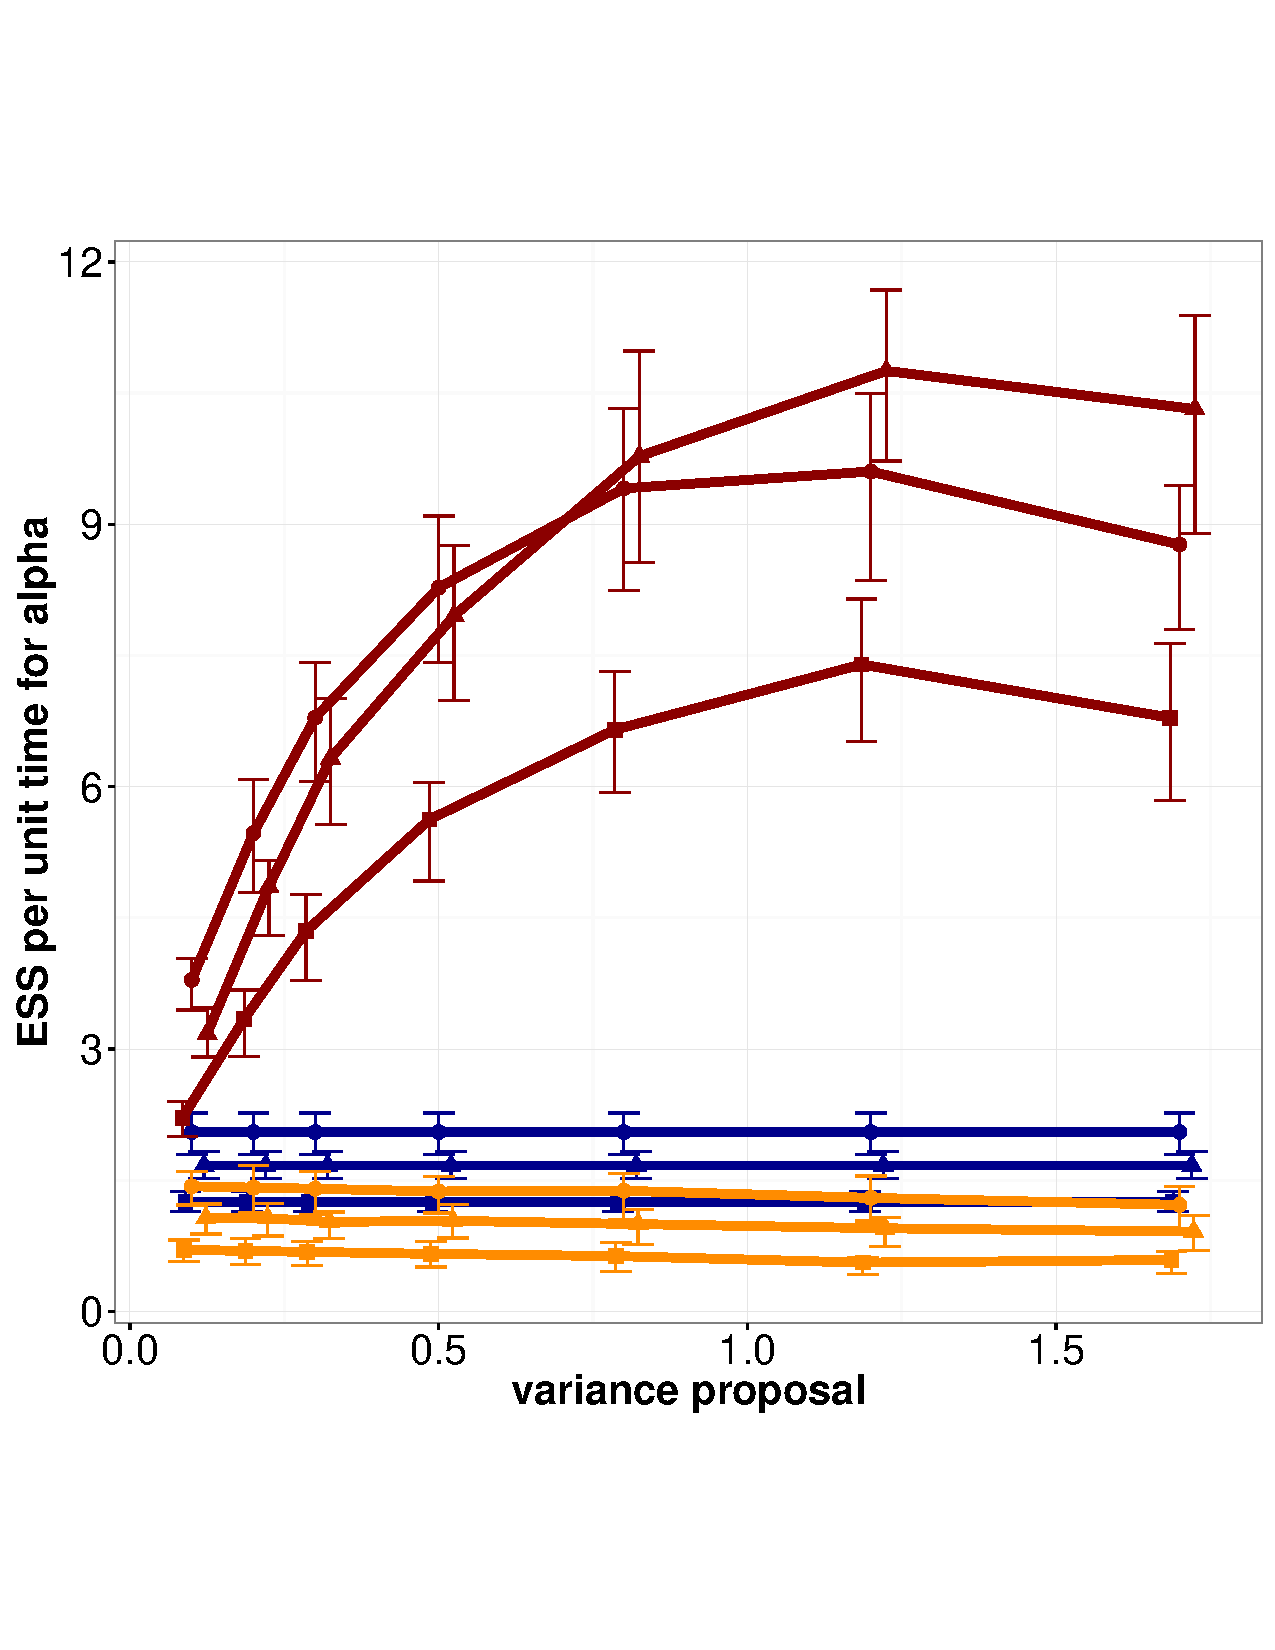
\includegraphics [width=0.70\textwidth, angle=0]{figs/jc.pdf}
    \vspace{-0.6in}
    \caption{ESS/sec for JC69 Model }
     \label{fig:ESS_JC}
  \end{minipage}
  \end{figure}
  The Jukes and Cantor (JC69) model is a popular model of DNA nucleotide
  substitution.  We write its state space as $\{0, 1, 2, 3\}$, representing the 
  four nucleotides $\{A, T, C, G\}$.  The model has a single parameter $\alpha$, 
  representing the rate at which the system transitions between any pair of 
  states. Thus, the rate matrix $A$ is given by 
  %Assume: $S = [S_0,S_1, ...,S_N] \;, T = [t_0(t_{start}), t_1,...,t_N, t_{N+1}(t_{end})]$, and y as observations.\\
$A_i = -A_{i,i} = 3\alpha, A_{i, j} = \alpha,i \neq j.$
We place a Gamma$(\alpha_0,\alpha_1)$ prior on the parameter $\alpha$.
%$$p(\alpha) = \frac{\lambda^\mu}{\Gamma(\mu)}\alpha^{\mu -1}e^{-\lambda \alpha} $$.
%Then we can get the posterior distribution $$f(\alpha | s_0,S,T)$$ as follows.
%$$ f(\alpha| s_0,S,T) \propto \exp(-(\lambda + 3(t_{end} - t_{start}))\alpha) \alpha^{\mu + N -1} .$$
%$\alpha | s_0,S,T$ is following $Gamma(\mu+ N,\lambda + 3(t_{end} - t_{start}))$\\


\subsection{Time-inhomogeneous immigration model with capacity}~
\vinayak{What is the prior over $w(t)$?}
We consider the Queuing model, with piece wise constant transition rate. 
\noindent Assume: $S = [S_0,S_1, ...,S_N] \;, T = [t_0(t_{start}), t_1,...,t_N, t_{N+1}(t_{end})]$, and y as observations.\\
Now, let's consider a immigration model as follows. State space is $\{0, 1, 2, ..., N - 1\}$, representing the total population. The transition matrix is defined as follows. 
% $$A_i(t) =: A_{i,i}(t) = -(\alpha + i\beta)w(t), \; \; i =0,1,...,N$$ $$A_{i, i+1}(t) = \alpha w(t), \; \; i =0,1,...,N-1,$$ $$A_{i, i-1}(t)  = \beta w(t), \; \;  i =1,...,N.$$
% $w(t)$ is a piece wise constant function. $w(t) = w_i, \; t \in [\l_i, l_{i + 1}), i = 1,2,3,..., K.$\\
% We already know the conditional density(given $\alpha,\; \beta$) of a MJP trajectory $(s_0, S, T)$ in time interval $[t_{start}, t_{end}]$, with $S=(s_1, s_2,..., s_k)$, $T=(t_1, t_2,..., t_k)$. 
% $$f(s_0,S,T| \alpha, \beta) = \prod_{i=0}^{k-1} A_{s_i, s_{i+1}}(t_i) \exp(\sum_{i=0}^{k} A_{s_i}(t_i)(t_{i+1} - t_{i})), $$
% where $t_0 = t_{start}$, $t_{k+1} = t_{end}.$\\
% Let's denote some notations here.\\
% $$U(s_0, S, T):= \sum_{i=0}^{k-1} \mathbb{I}_{\{s_{i+1} - s_i = 1\}}.$$
% $$D(s_0, S, T):= \sum_{i=0}^{k-1} \mathbb{I}_{\{s_{i+1} - s_i = -1\}}.$$
% Call them U and D for short.
% Let's denote the total time when the trajectory state stays at state i as $\tau_i$, i.e. $\tau_i = \sum_{j=0}^{k} (t_{j+1} -t_j)\mathbb{I}_{\{s_j = i\}}$, then $\sum_{i=0}^k (t_{i+1} - t_i)s_i = \sum_{i=0}^N \tau_ii.$\\

% $$f(s_0,S,T| \alpha, \beta) \propto \exp(\sum_{r = 0}^{K}-w_r\alpha(l_{r + 1} - l_{r}- \tau_N^r) )\alpha^U \cdot  \exp(-\int_{t_s}^{t_{e}}(S(t)w(t)\beta)  \beta^D$$\\
% If we assume the prior of $\alpha$, and $\beta$ are $Gamma(\mu,\lambda)$, $Gamma(\omega, \theta)$, which are independent with each other. \\
% $$p(\alpha) = \frac{\lambda^\mu}{\Gamma(\mu)}\alpha^{\mu -1}e^{-\lambda \alpha}. $$
% $$p(\beta) = \frac{\theta^\omega}{\Gamma(\omega)}\beta^{\omega -1}e^{-\theta \beta}. $$
% Then we can get the posterior distribution $$f(\alpha, \beta | s_0,S,T)$$ as follows.
% $$ f(\alpha, \beta | s_0,S,T) \propto \exp(-(\lambda +\sum_{r = 0}^{K}w_r\alpha(l_{r + 1} - l_{r}- \tau_N^r))\alpha) \alpha^{\mu + U -1} \cdot \exp(-(\int_{t_{s}}^{t_{e}}(S(t)w(t) + \theta)\beta) \beta^{\omega+ D -1}.$$
% It means that the posterior distributions of $\alpha$, $\beta$ are still independent. \\
% $\alpha | s_0,S,T$ is following $Gamma(\mu+ U,\lambda +\sum_{r = 0}^{K}w_r\alpha(l_{r + 1} - l_{r}- \tau_N^r)  )$\\
% $\beta | s_0,S,T$ is following $Gamma(\omega+ D,\int_{t_s}^{t_{e}}(S(t)w(t) + \theta)$.\\
% Such immigration models have perfectly conjugate posterior distributions when we assign $\gamma$ priors to $\alpha$ and $\beta$. We apply our Metropolis Hasting algorithms on such models to compare the performance with the performance of Gibbs Sampling algorithm.

\subsection{Experiments}

 In Figure~\ref{fig:ESS_pc_3}, Figure~\ref{fig:ESS_pc_5}, Figure~\ref{fig:ESS_pc_10}, we plot the ESS per unit time for the parameters $\alpha$ (left) and $\beta$ (right) as we change the variance of the
  proposal kernel per run, for different methods and different scaling parameters k($k = 1.5, 2, 3$) and different dimensions($p = 3, 5, 10$), where   $k = 1.5$,  $\Omega(\theta, \theta^*) = k \max(\max A(\theta), \max A(\theta^*))$. Blue lines are for Gibbs sampler. Red lines are for improved MH. Orange lines are for naive MH. Black lines are for particle MCMC. Lines with dots correspond to $k = 1.5$. Lines with triangle correspond to $k = 2$. Lines with squares correspond to $k = 3$. For $k=$ $2$ or $3$, $\Omega(\theta, \theta^*) = \frac{k}{2} (\max A(\theta) + \max A(\theta^*))$. We see that the improved MH algorithm is more efficient i	n these cases with respect to the overall ESS per unit time. We also see that increase the scaling parameter will decrease the efficiency of the improved MH algorithm respect to overall ESS per unit time, when $k > 2$. If we set $\Omega = 1.5 \max(\Omega_{old}, \Omega_{new})$, the performance of the improved MH will not be as good as the case we set $\Omega = 2(\Omega_{old} + \Omega_{new})$ when the proposal log variance is large.\\

  \begin{figure}%[b]
  \centering
  \begin{minipage}[!hp]{0.45\linewidth}
  \centering
    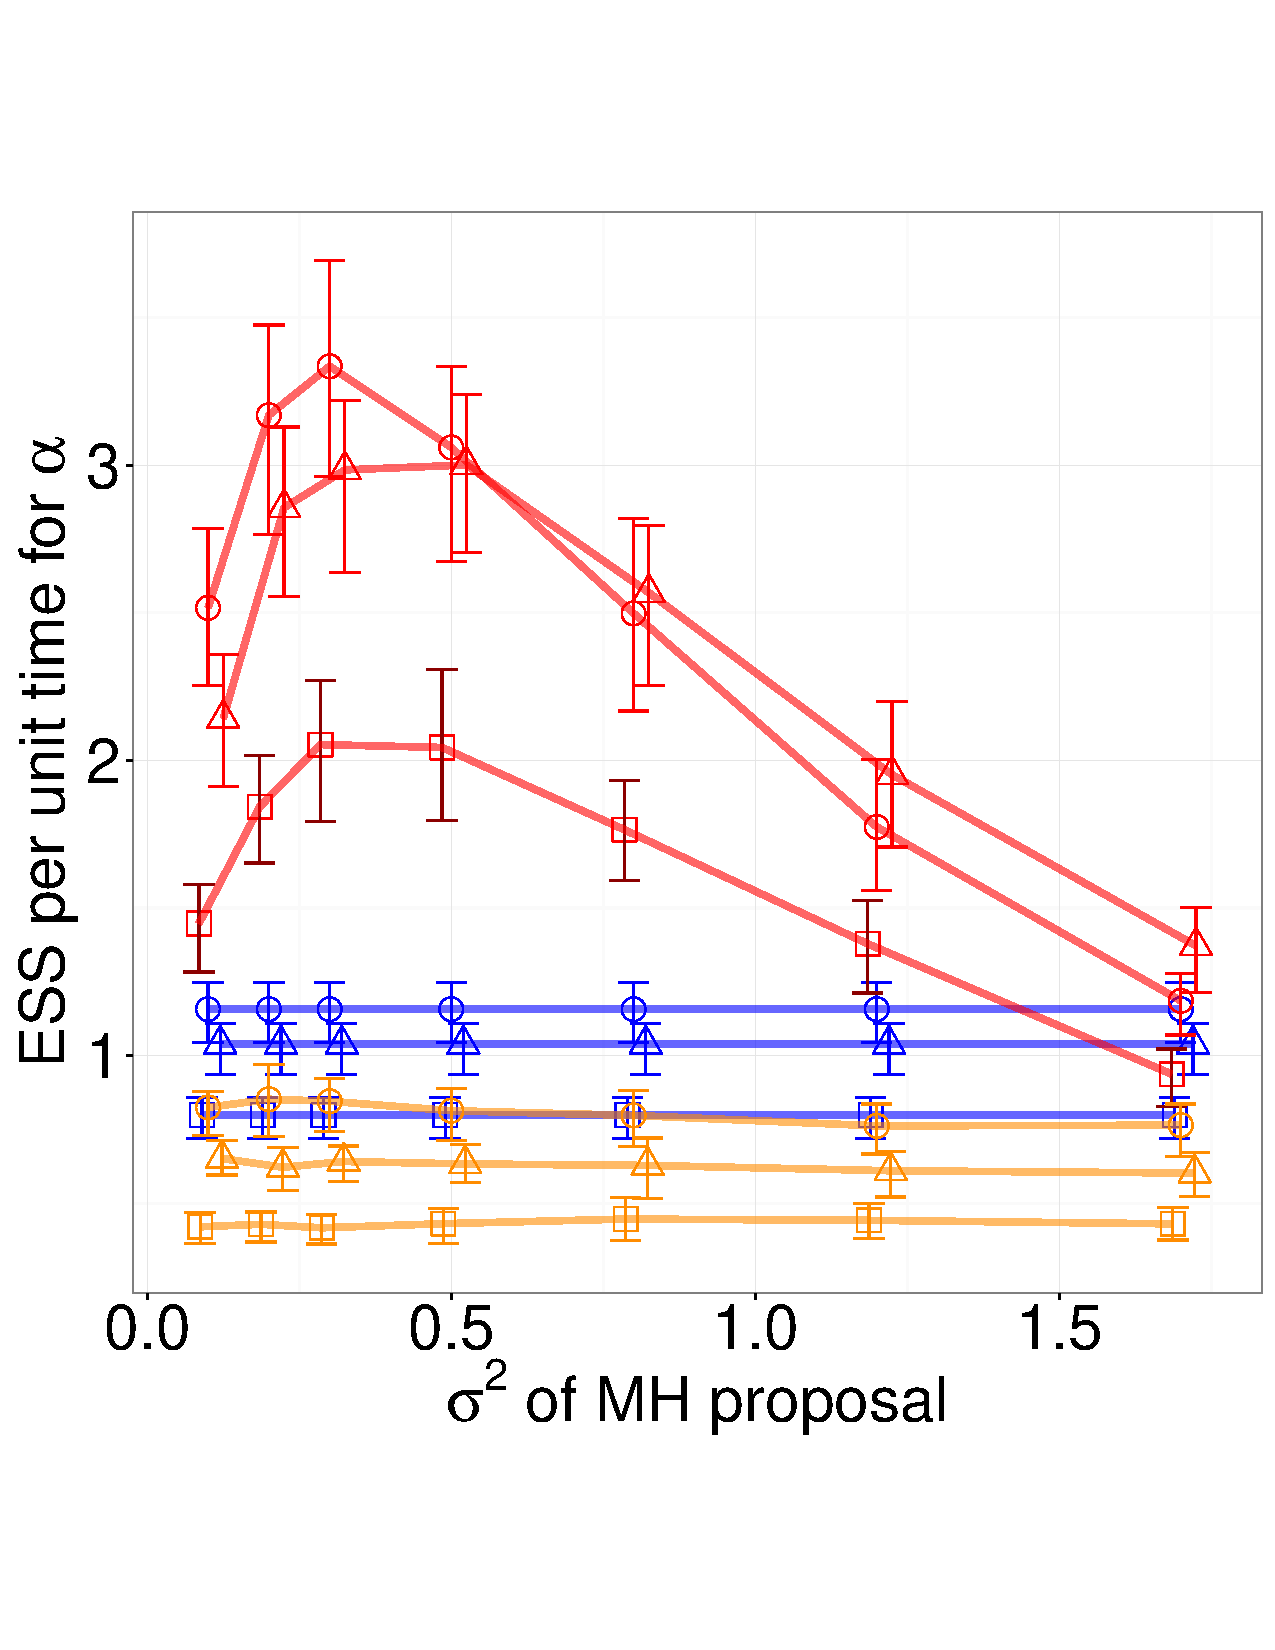
\includegraphics [width=0.70\textwidth, angle=0]{figs/pc_3_alpha.pdf}
      \end{minipage}
  \begin{minipage}[!hp]{0.45\linewidth}
  \centering
    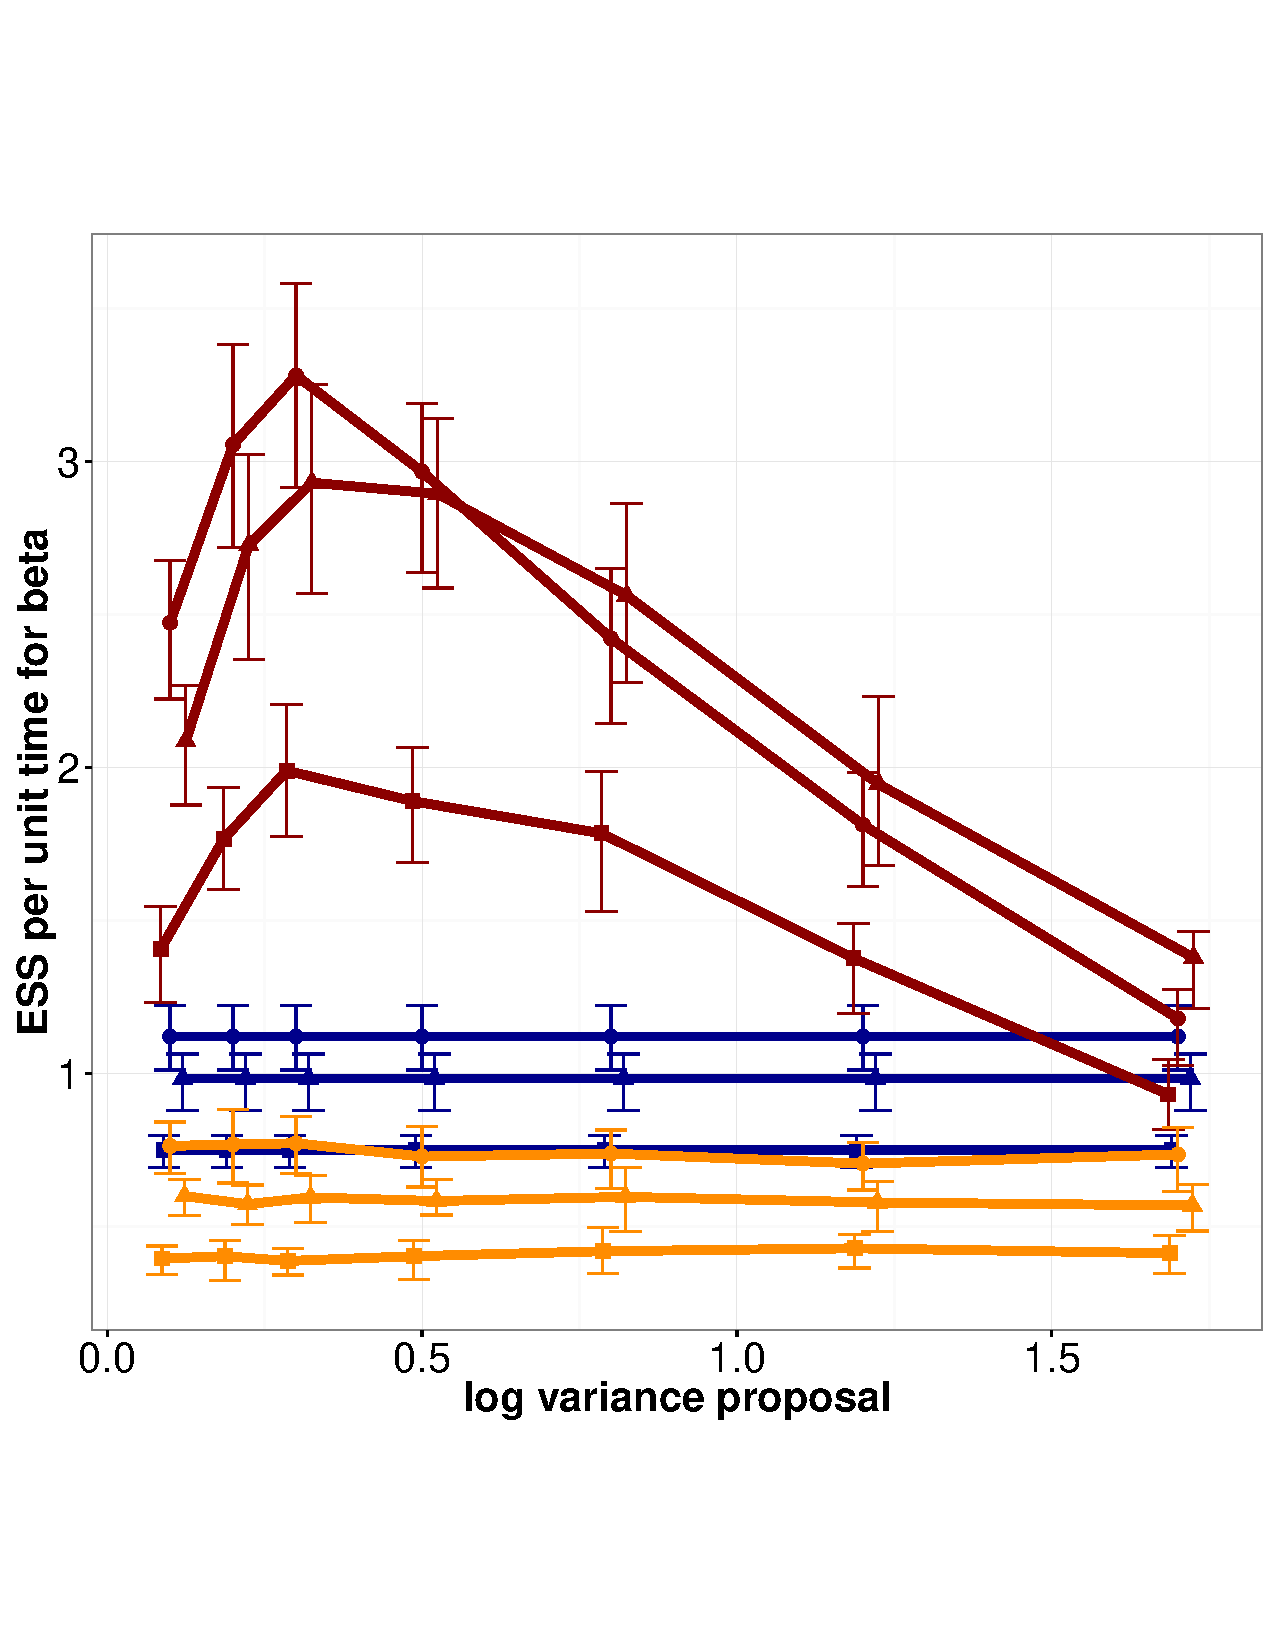
\includegraphics [width=0.70\textwidth, angle=0]{figs/pc_3_beta.pdf}
    \vspace{-0 in}
     \label{fig:ESS_pc_3}
  \end{minipage}
    \caption{ESS/sec for NH Immigration model (dim 3)}
  \end{figure}

  \begin{figure}%[b]
  \centering
  \begin{minipage}[!hp]{0.45\linewidth}
  \centering
    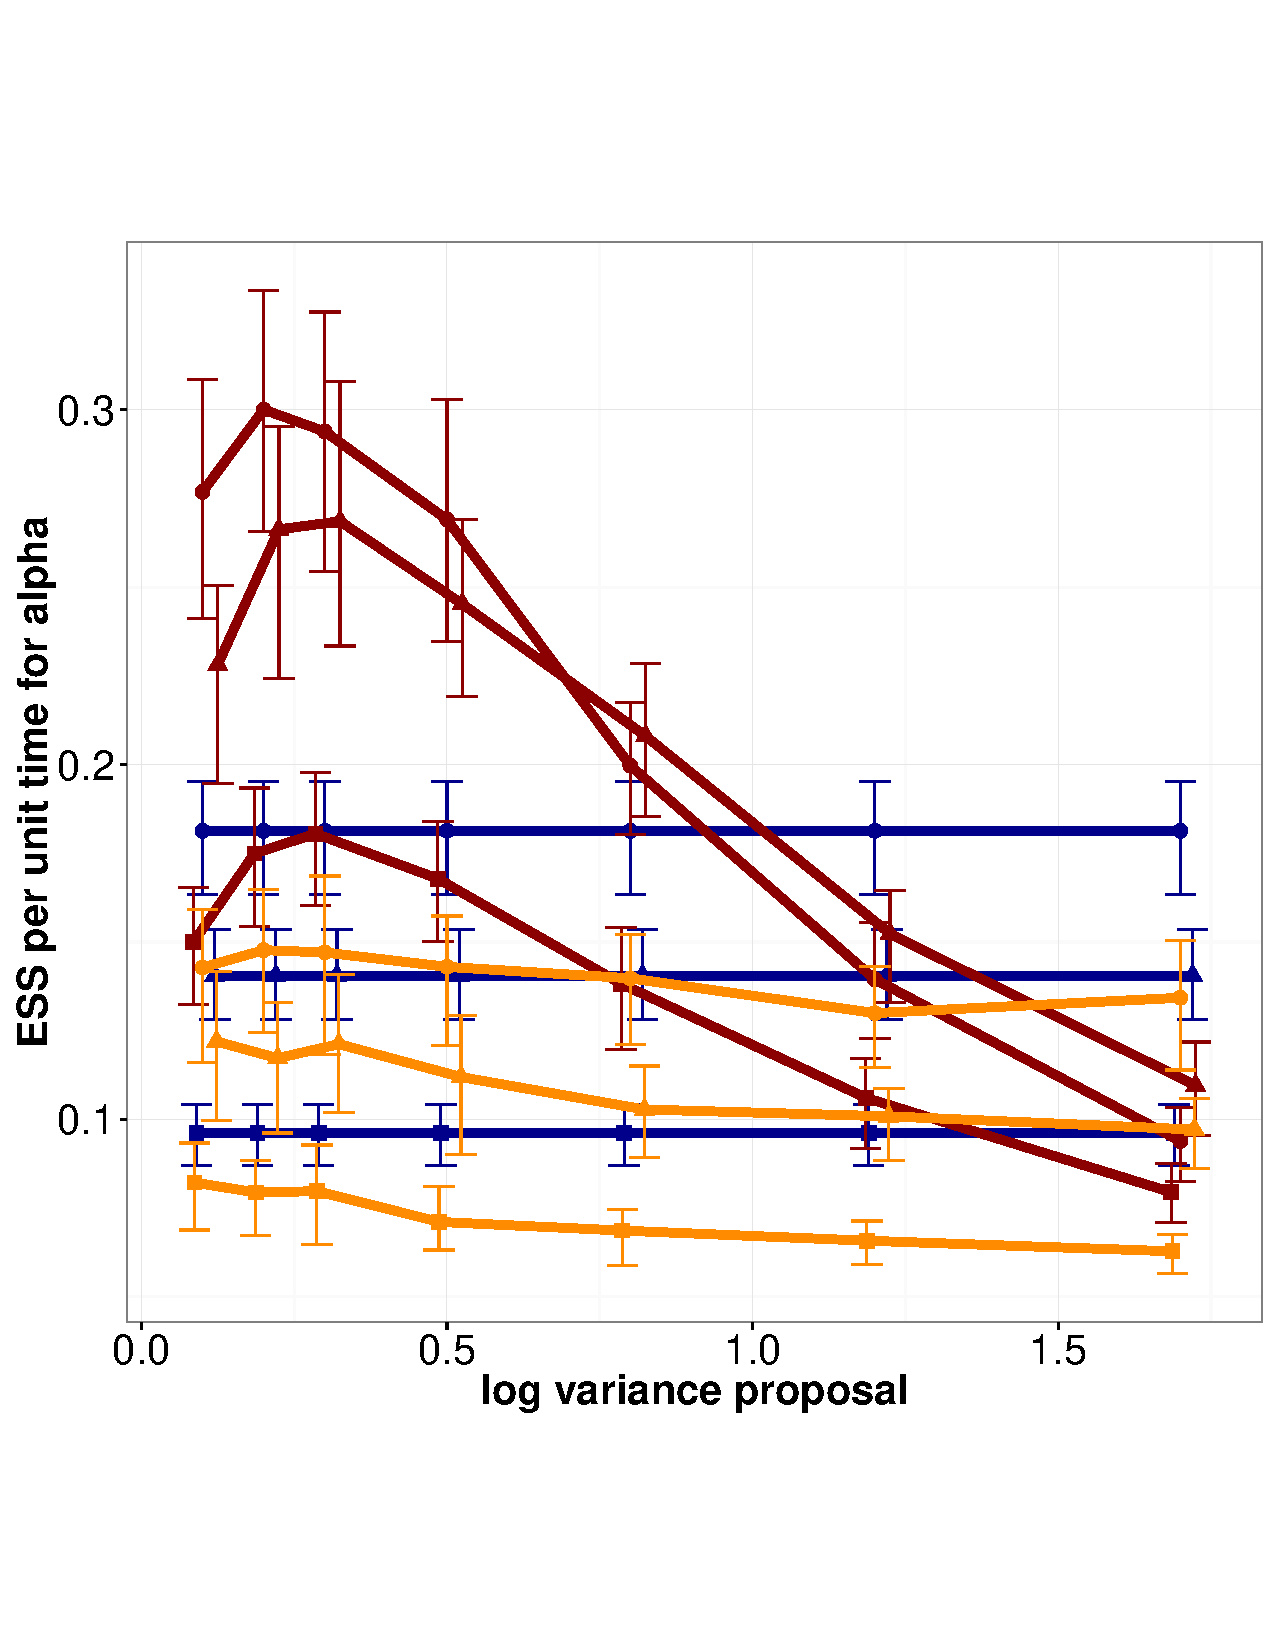
\includegraphics [width=0.70\textwidth, angle=0]{figs/pc_10_alpha.pdf}
      \end{minipage}
  \begin{minipage}[!hp]{0.45\linewidth}
  \centering
    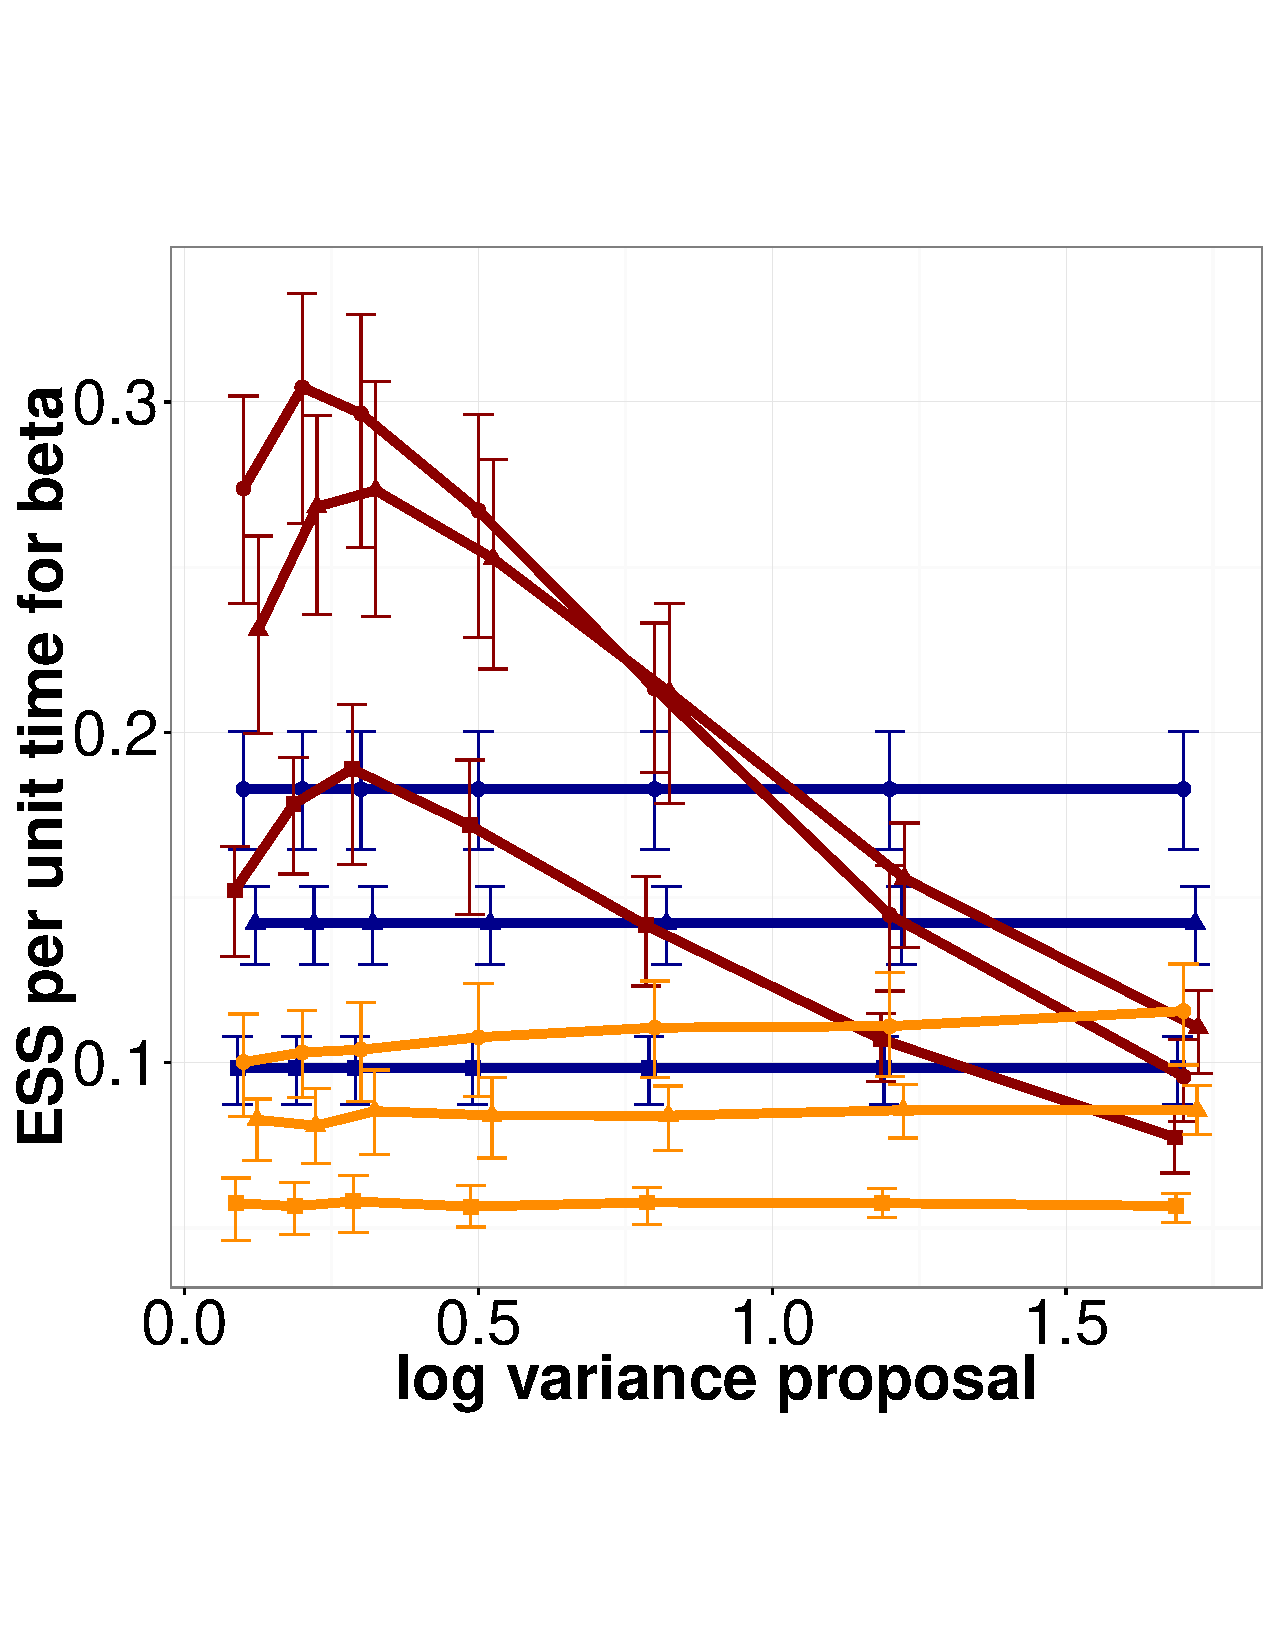
\includegraphics [width=0.70\textwidth, angle=0]{figs/pc_10_beta.pdf}
    \vspace{-0 in}
  \end{minipage}
     \label{fig:ESS_pc_10}
    \caption{ESS/sec for NH Immigration model (dim 10)}
  \end{figure}
